% ========================================= TEMPLATE INFO ========================================
%
% Author:       P4ntomime
% Version:      1.0.0
% Last updated: 2024-02-18
% Brief:        A LaTeX template for summaries. See README.md for more information.
% 
% ================================================================================================
\documentclass[8pt, a4paper, twoside, landscape]{extarticle}
% Font size:    8pt
% Paper size:   A4
% style:        twoside (needed, so odd and even pages have different margins)
% orientation:  portrait. (use 'landscape' for landscape orientation)


% ========================================= DOCUMENT INFO =========================================
\def\title{KomFour}       % title
\def\shorttitle{KomFour}                            % short title (displayed as PDF title)
\def\dozent{Remo Bernhardsgrütter}                  % lecturer
\def\semester{FS 2026}                              % semester
\def\author{Simone Stitz, Mirko Ratti}                           % author(s)
\def\repo{https://gitlab.com/sstitz/komfour}        % repository link
\def\version{3.0.\today}                            % version
\def\pagelimit{6}                                   % page limit -> causes pages after limit to be red
\def\titleoption{ultra compact}                     % options: ultra compact, compact, normal
\def\enableToC{false}

% ================================= PACKAGES, SETUP AND COMMANDS ==================================
\input{preamble.tex}


% =========================================== DOCUMENT ============================================
\begin{document}
    \begin{layout}
        \section{Komplexe Zahlen}

\subsection{Darstellungsformen von komplexen Zahlen}

\subsubsection{Normalform (kartesisch)} 

\vspace{-0.2cm}

$$ z = z_1 + \, \jimg z_2 \qquad z_1 = \RE(z) \qquad z_2 = \IM(z) \qquad \vert z \vert = \sqrt{z_1^2 + z_2^2} $$
\vspace{-2em}

$$ \RE(z) = \frac{1}{2}(z+\overline{z}) \qquad \qquad \IM(z) = \frac{1}{2\jimg}(z - \overline{z})$$

\para{Umrechnung in Polarform ($r, \varphi$)} 

\vspace{-0.2cm}

$$ r =  \vert z \vert = \sqrt{z_1^2 + z_2^2} \qquad 
\varphi = \begin{cases} 
\arctan\left(\frac{z_2}{z_1}\right), & z_1 > 0 \\ 
\arctan\left(\frac{z_2}{z_1}\right) + \pi, & z_1 < 0 
\end{cases} = \begin{cases} 
\arccos\left(\frac{z_1}{r}\right), & z_2 \geq 0 \\ 
-\arccos\left(\frac{z_1}{r}\right), & z_2 < 0 
\end{cases}$$


\subsubsection{Polarform / \cbl{Eulerform}}

\vspace{-0.2cm}

$$ z = r \cdot \cjs(\varphi) = r \cdot \left(\cos(\varphi) + \jimg \sin(\varphi)\right) = \cbl{r \cdot \e^{ \jimg \varphi}} \qquad \varphi = \arg(z) $$


\para{Umrechnung in Normalform (kartesisch)}\vspace{-0.2cm}

$$ \RE(z) = z_1 = \vert z \vert \cdot \cos(\varphi) \qquad \qquad \IM(z) = z_2 = \vert z \vert \cdot \sin(\varphi) $$ 

\subsubsection{Wichtige Zusammenhänge}\vspace{-0.5cm}

\[\jimg^2 = -1 \qquad \frac{1}{\jimg} = -\jimg \qquad \e^{\jimg \, \pi} = -1 \qquad
\e^{\jimg \frac{\pi}{2}} = \jimg \qquad \jimg^{\jimg} = \e^{- \frac{\pi}{2} + 2k \pi} \qquad | \cjs(\varphi)| = 1 \]

\[e^{\jimg \varphi} = \cjs(\varphi) \qquad \cjs(\alpha) \cdot \cjs(\beta) = \cjs(\alpha + \beta) \qquad \cjs(\alpha) : \cjs(\beta) = \cjs(\alpha - \beta)\]

$$z_1 \perp z_2 \Leftrightarrow \RE\left(\frac{z_1}{z_2}\right) = 0 \Leftrightarrow \arg\left(\frac{z_1}{z_2}\right) = \pm \frac{\pi}{2}$$

\subsubsection{Geometrische Aspekte von komplexen Zahlen}

\begin{minipage}[t]{0.47\columnwidth}
    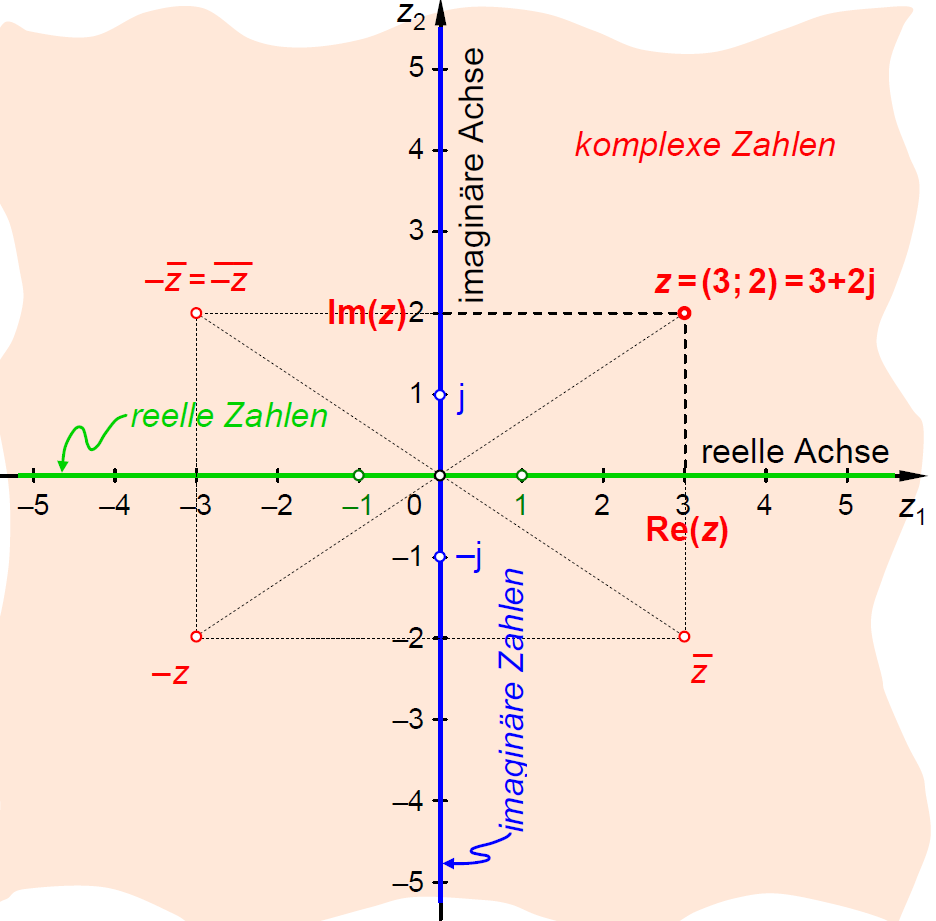
\includegraphics[width=\linewidth, align=t]{images/komplexe_zahlen_uebersicht.png}
\end{minipage}
\hfill
\begin{minipage}[t]{0.47\columnwidth}
    \para{komplex-konjugieren}

    \textrightarrow\ Spiegelung an \textbf{reeller} Achse

    $$z = 3 + 2\jimg \quad \rightarrow \quad \overline{z} = 3 - 2\jimg$$
    \vspace{1em}

    \renewcommand{\arraystretch}{1.5}
    \begin{tabular}{l c l}
        $\overline{a + b} = \overline{a} + \overline{b}$            & & $\overline{a - b} = \overline{a} - \overline{b}$          \\ 
        $\overline{a \cdot b} = \overline{a} \cdot \overline{b}$    & & $\overline{a \div b} = \overline{a} \div \overline{b}$
    \end{tabular}
    \renewcommand{\arraystretch}{1}

    \medskip
    \medskip

    \para{Multiplikation mit $\bm{(-1)}$}

    \textrightarrow\ Punktspeigelung am Ursprung

\end{minipage}


\subsection{Rechenoperationen}

\subsubsection{Addition / Subtraktion}

Gleiches Vorgehen wie in $\mathbb{R}$ (\textbf{kartesisch})

\smallskip

\renewcommand{\arraystretch}{1.4}
\begin{tabular}{ll}
    Addition:       & $(a_1 + \jimg a_2) + (b_1 + \jimg b_2) = (a_1 + b_1) + \jimg (a_2 + b_2)$ \\
    Subtraktion:    & $(a_1 + \jimg a_2) - (b_1 + \jimg b_2) = (a_1 - b_1) + \jimg (a_2 - b_2)$ 
\end{tabular}
\renewcommand{\arraystretch}{1}


\subsubsection{Multiplikation}

\renewcommand{\arraystretch}{1.4}
\begin{tabular}{ll}
    kartesisch:     & $(a_1 + \jimg a_2) \cdot (b_1 + \jimg b_2) = (a_1 b_1 - a_2 b_2) + \jimg (a_1 b_2 + a_2 b_1)$ \\
    \textbf{polar:} & $a \cdot b = \vert a \vert \vert b \vert \, e^{\jimg (\varphi_1 + \varphi_2)}$                \\
                    & \textrightarrow\ Beträge multiplizieren und Argumente (Winkel) addieren
\end{tabular}
\renewcommand{\arraystretch}{1}

La moltiplicazione equivale ad una rotazione di angolo $\arg(b)$ e una streckung di $\vert b \vert$.

\subsubsection{Division}

\renewcommand{\arraystretch}{1.6}
\begin{tabular}{ll}
    kartesisch:     & $\frac{(a_1 + \jimg a_2)}{(b_1 + \jimg b_2)} = 
                    \frac{(a_1 + \jimg a_2) \cbl{(b_1 - \jimg b_2)}}{(b_1 + \jimg b_2) 
                    \cbl{(b_1 - \jimg b_2)}} = \frac{\text{ausmultiplizieren}}{b_1^2 + b_2^2}$ 
                    \qquad {\small$\color{blue}\blacksquare$: Konjugiert komplexe}\\
    \textbf{polar:} & $\frac{a}{b} = \frac{\vert a \vert}{\vert b \vert} \, \e^{\jimg (\varphi_1 - \varphi_2)}$                                                                                                    \\
                    & \textrightarrow\ Beträge dividieren und Argumente (Winkel) subrahieren
\end{tabular}
\renewcommand{\arraystretch}{1}

\smallskip

\textbf{Hinweis:} Es gilt: $\Big| \frac{a}{b} \Big| = \frac{\vert a \vert}{\vert b \vert}$ 


\subsubsection{Potenzieren (De Moivre)}

\textbf{Potenzgesetze gelten weiterhin für \myul{ganzzahlige} Exponenten!}

\[z^n = r^n \cdot \big[ \cos(\alpha) + \jimg \sin(\alpha) \big]^n = r^n \cdot \big[ \cos(n \alpha) + \jimg \sin(n \alpha) \big] \qquad \text{ für } n \in \mathbb{N} \]

Mit der Formel von de Moivre können \textbf{Mehrfachwinkelformeln} aus der Trigo hergleitet
werden:\vspace{-1em}

\begin{center}
    \begin{tabular}{cl}
        $\underbrace{[\cos(\zeta) + \jimg \sin(\zeta)]^2} $ & $= {\color{green}\cos(2\zeta)} + \jimg {\color{blue}\sin(2\zeta)}$ \\
        $= [\cos(\zeta)]^2 + 2\jimg \cos(\zeta)\sin(\zeta) + \jimg^2 [\sin(\zeta)]^2$ &\\
        $= [{\color{green}\cos(\zeta)}]^2 - [{\color{green}\sin(\zeta)}]^2 + \jimg \cdot {\color{blue}2 \sin(\zeta) \cos(\zeta)} $&
    \end{tabular}
\end{center}

% 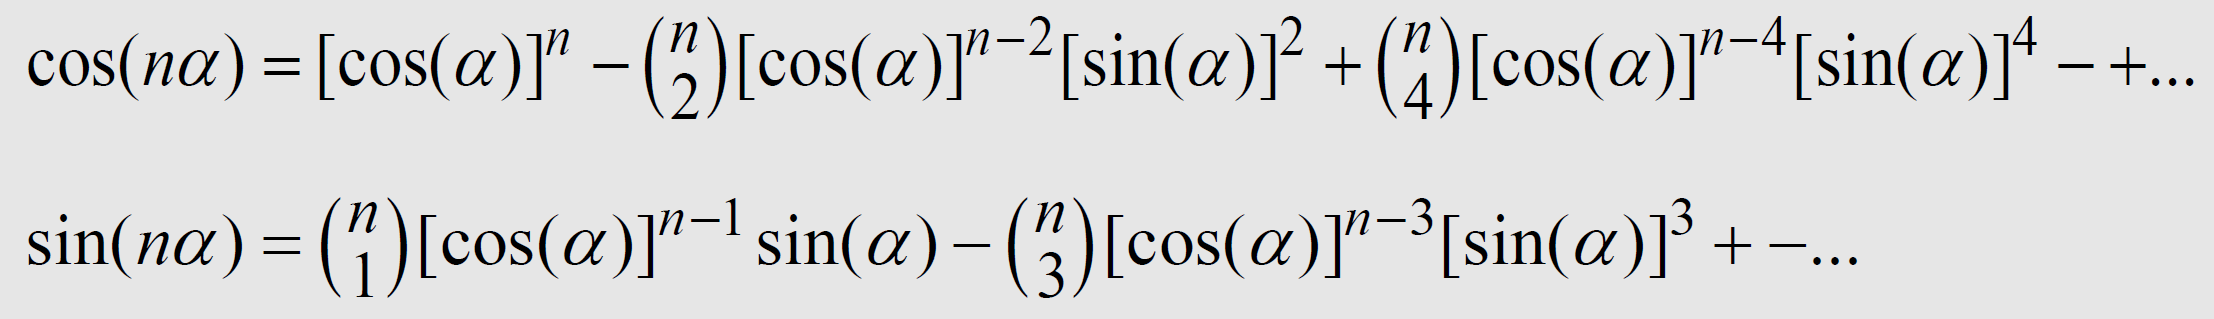
\includegraphics[width=\columnwidth]{images/mehrfachwinkel_2.PNG}
\subsubsection{Estrazione di radice $n$-esima (Radicazione)}

\begin{itemize}
    \item \textbf{Proprietà:} Le distributive delle radici \textbf{non si estendono} generalmente al campo complesso ($\sqrt{ab} \neq \sqrt{a}\sqrt{b}$ in $\mathbb{C}$).
    \item \textbf{Molteplicità:} Ogni numero complesso $a \neq 0$ ammette esattamente $n$ radici $n$-esime distinte in $\mathbb{C}$.
    \item \textbf{Geometria:} Le soluzioni si dispongono nel piano come i vertici di un \textbf{$n$-agono regolare} centrato nell'origine e inscritto in una circonferenza di raggio $R = \sqrt[n]{|a|}$.
\end{itemize}\vspace{-0.8em}

\[z^n = a \implies z_k = \sqrt[n]{|a|} \left( \cos \frac{\varphi + 2k\pi}{n} + \jimg \sin \frac{\varphi + 2k\pi}{n} \right), \quad k \in \{0, 1, \dots, n-1\}\]\vspace{-0.5em}
% \[z^n = a  \qquad \vert z \vert = \sqrt[n]{\vert a \vert} \qquad \qquad \arg(z_1) = \frac{\arg(a)}{n} \qquad \arg(z_n) = \frac{\arg(a)}{n}+k\cdot \frac{2\pi}{n}\]

\example{Determinazione delle radici quarte di $-16$ ($z^4 = -16$)}

\begin{minipage}{0.58\columnwidth}
    \begin{enumerate}
        \item \textbf{Modulo ($|z_k|$):}
        \begin{align*}
            \lvert z \rvert^4 \cdot \cjs(4 \varphi) &= 16 \cdot \cjs(\pi)\\
            z = \sqrt[4]{\lvert 16 \rvert} &= 2
        \end{align*}
        \item \textbf{Argomento principale ($z_0$):}
    
        Si divide l'argomento $\arg(a) = \pi$ per l'indice $n=4$:
        \begin{equation*}
            \alpha_0 = \frac{\arg(a)}{n} = \frac{\pi}{4} = 45^\circ
        \end{equation*}
        \item \textbf{Argomenti successivi:}
        Si applica un incremento angolare costante $\Delta\varphi = \frac{2\pi}{n} = \frac{\pi}{2}$:
        \begin{align*}
            \alpha_1 &= \frac{\pi}{4} + \frac{\pi}{2} = \frac{3\pi}{4} \\
            \alpha_2 &= \frac{3\pi}{4} + \frac{\pi}{2} = \frac{5\pi}{4} \\
            \alpha_3 &= \frac{5\pi}{4} + \frac{\pi}{2} = \frac{7\pi}{4}
        \end{align*}
    \end{enumerate}    
\end{minipage}
\hfill
\begin{minipage}{0.38\columnwidth}
    \centering
    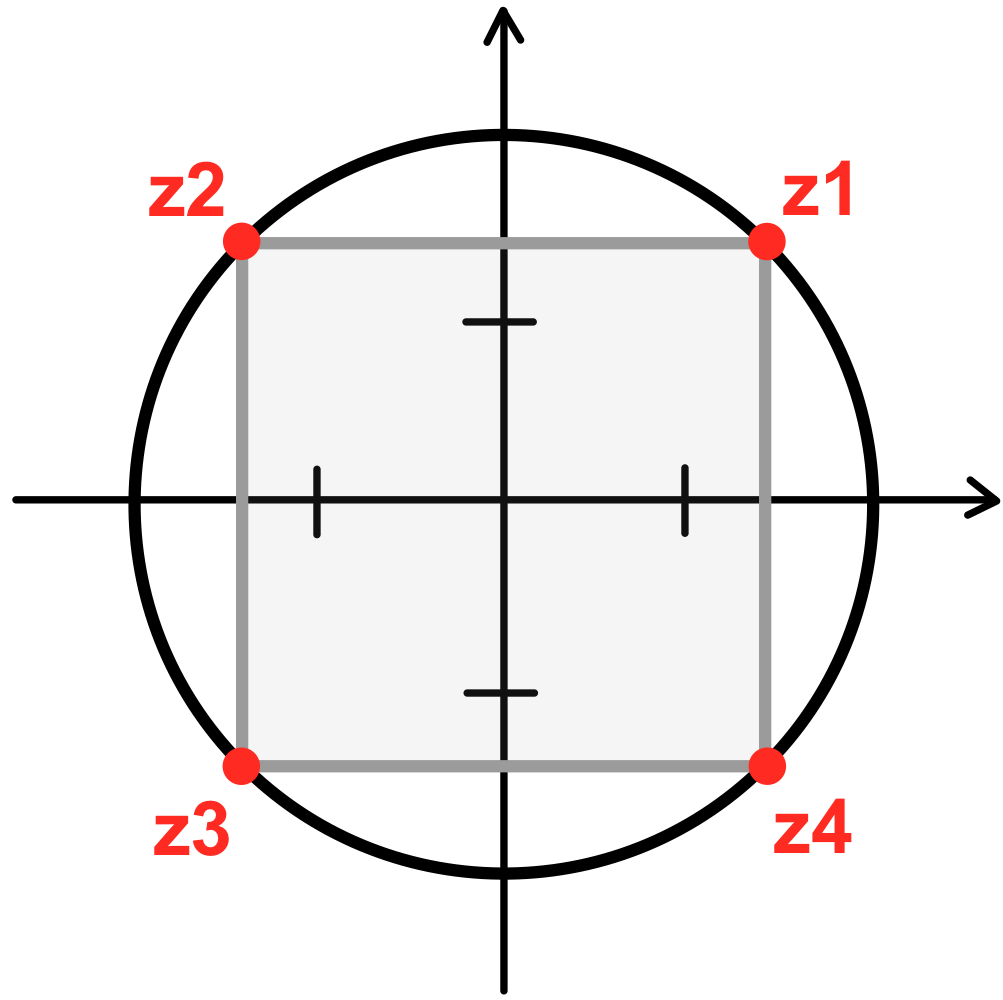
\includegraphics[width=\linewidth]{images/wurzel.png}
    \begin{align*}
        z_0 &= \sqrt{2} + \jimg\sqrt{2} \\
        z_1 &= -\sqrt{2} + \jimg\sqrt{2} \\
        z_2 &= -\sqrt{2} - \jimg\sqrt{2} \\
        z_3 &= \phantom{-}\sqrt{2} - \jimg\sqrt{2}
    \end{align*}
\end{minipage}

% Versione ottimizzata del formalismo di Steiner
Posto $a = r \mathrm{e}^{\jimg \varphi}$, l'insieme delle radici $n$-esime è definito come:
\begin{equation*}
    \mathcal{S} = \left\{ \sqrt[n]{r} \cdot \mathrm{e}^{\jimg \left( \frac{\varphi}{n} + \frac{2k\pi}{n} \right)} \;\middle|\; k \in \mathbb{Z}, \, 0 \le k < n \right\}
\end{equation*}
\para{Einheitswurzel $\bm{\sqrt[n]{1}}$}		

Durch Multiplikation mit der $n$-ten Einheitswurzel erreicht man eine reine Drehung um $\frac{360}{n}$ Grad im \textbf{Gegenuhrzeigersinn}. \\	
\textbf{Achtung!} Die erste Lösung von $\sqrt[n]{1}$ ist immer die reelle Zahl 1\\
\textrightarrow\ nächste Lösung verwenden!

\begin{center}
    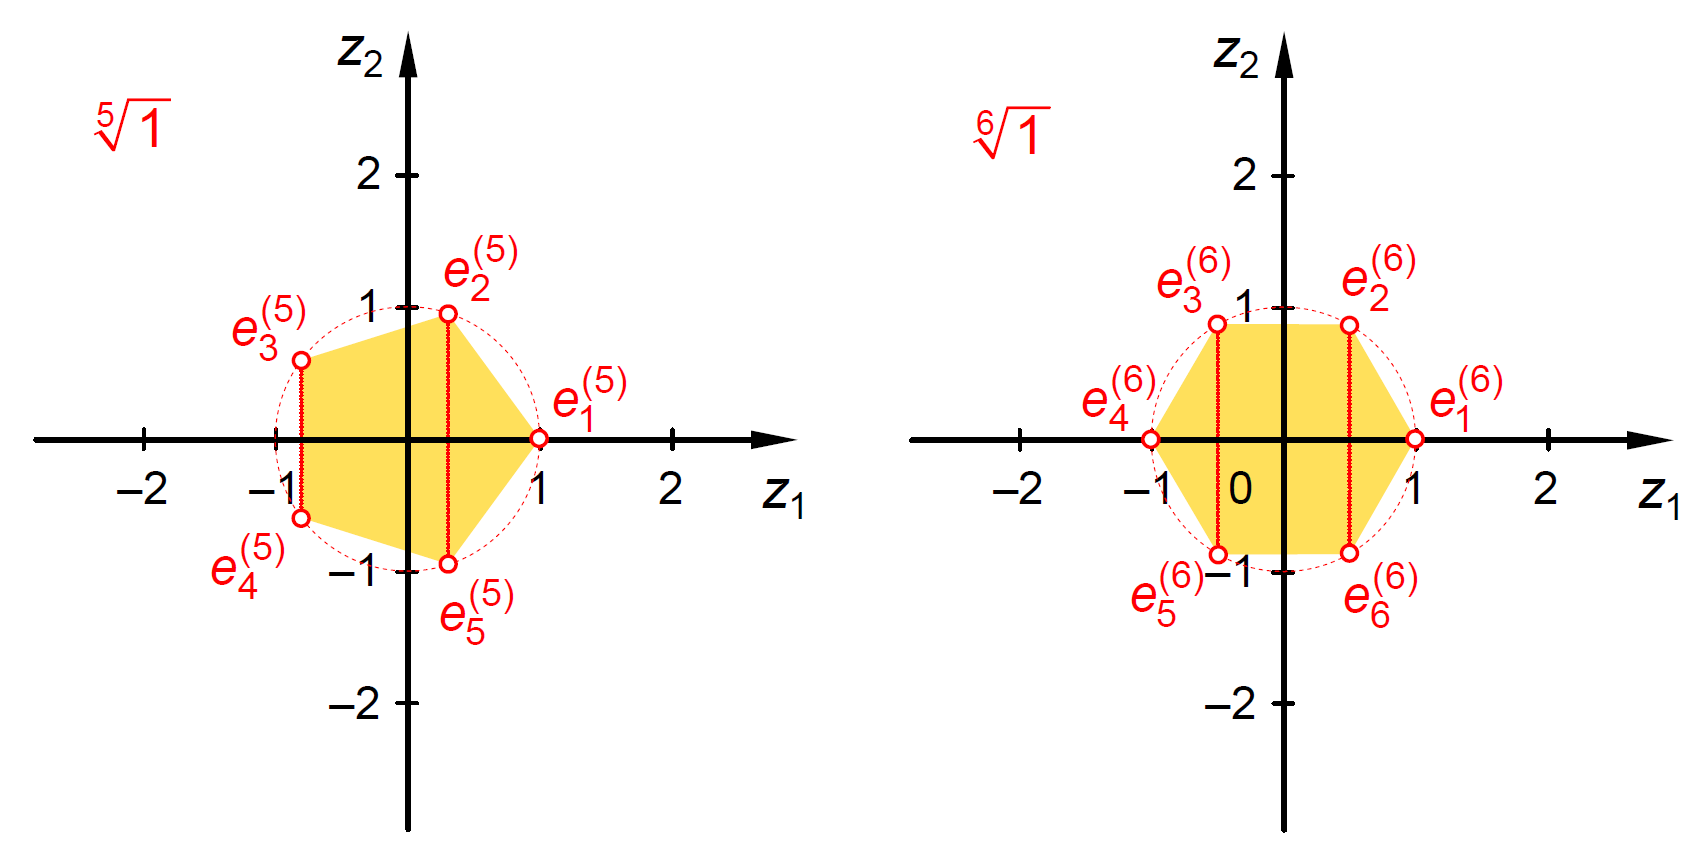
\includegraphics[width=0.9\columnwidth]{images/einheitswurzel.PNG}
\end{center}

\subsubsection{Komplexwertige Exponentialfunktion}

\vspace{-0.2cm}

\[\e^z = \e^{z_1 + \jimg z_2} = \e^{z_1} \cdot \e^{\jimg z_2} = \e^{z_1} \cdot \cjs(z_2) \qquad \rightarrow \qquad \boxed{e^{\jimg \varphi} = \cjs(\varphi)}\]

\textrightarrow\ Die Exponentialfunktion ist $2 \pi \jimg$-periodisch (auf imaginärer Achse)

\medskip

\para{Exponentialgesetze}

Die Exponentialgesetze bleiben in $\mathbb{C}$ für \myul{ganzzahlige} Exponenten erhalten!

\smallskip

\begin{tabular}{l c l c l}
    $\e^a \cdot \e^b = \e^{a+b}$    & & $\e^a : \e^b = \e^{a-b}$    & & $a, \; b \in \mathbb{C}$    \\
    $(\e^a)^k = \e^{ka}$            & &                             & & $k \in \mathbb{Z}$
\end{tabular}


\example{Exponentialfunktion}

\begin{itemize}
    \item $\e^z = e^{\cor{1}\cbl{-\frac{\pi}{2}} \jimg} = \e^{\cor{1}} \cdot \cjs(\cbl{- \frac{\pi}{2}}) = \e \cdot (- \jimg) = -2.781 \jimg$
    \item $\e^z = \e^{\cor{\ln(2)} + \cbl{3 \pi} \jimg} = \e^{\cor{\ln(2)}} \cdot \cjs(\cbl{3 \pi}) = 2 \cdot \cjs(\pi) = -2$ 
\end{itemize}



\subsubsection{Komplexwertige Logarithmusfunktion}

\textbf{\crd{Ehemalige Log-Gesetze sind nur noch Kongruenzgesetze!}}

\[ \Ln(z) = \ln(\vert z \vert) + \jimg (\arg(z)+ \cor{k2\pi}) \qquad (z \in \mathbb{C}, \, z \neq 0, k \in \mathbb{Z})\]

\textrightarrow\ Die Exponentialfunktion ist $\cor{2 \pi \jimg\text{-periodisch}}$ ($\infty$ viele lösungen)

    

\subsubsection{Allgemeine Potenzfunktion}

\textbf{\crd{Es existieren keine Potenz- oder Kongruenzgesetze!}} 
\[a^b = \e^{b \cdot \Ln(a)} \qquad (a, \; b \in \mathbb{C}, \; a \neq 0)\]


\subsubsection{Komplexwertige Trigonometrische Funktionen}

\vspace{-0.2cm}

\[\sin(\alpha \cdot z) = \frac{\e^{\alpha \jimg z} - \e^{-\alpha \jimg z}}{2 \jimg} \qquad 
\cos(\alpha \cdot z) = \frac{\e^{\alpha \jimg z} + \e^{-\alpha \jimg z}}{2} \qquad 
\tan(z) = \frac{\e^{\jimg z} - \e^{-\jimg z}}{\jimg(\e^{\jimg z} + \e^{-\jimg z})}\]


\subsection{Polynome (vgl. Radizieren)}
Alle Nullstellen des Polynoms $p(z) = a_n z^n + a_{n-1}z^{n-1} + \ldots + a_0$ liegen in der Gauss'schen Zahlenebene in einer
Kreisscheibe um den Ursprung mit Radius $\sum\limits _{k=0}^n \bigl| \frac{a_k}{a_n} \bigl|$

\smallskip

Für Gleichungen vom Grad $\geq$ 5 existieren \textbf{keine} nur aus den 4 Grundoperationen und Wurzeln zusammengesezten Lösungsformeln.	


\subsubsection{Polynome mit Koeffizienten $\bm{\in \mathbb{C}}$}

Wichtige Eigenschaften von komplexen \textbf{und} reellen Polynomen:

\smallskip

\begin{enumerate}[itemsep=0.2cm]
    \item Jedes komplexe Polynom vom Grad $\geq 1$ hat in $\mathbb{C}$ mindestens eine Nullstelle
    \item Ein komplexes Polynom vom Grad $n$ zerfällt in $\mathbb{C}$ in lauter Linearfaktoren. \\
        Die Faktoren müssen \textbf{nicht} verschieden sein.
        Die Zerlegung ist bis auf die Reihenfolge eindeutig. \\
        Beispiel: $a_n z^n + a_{n-1}z^{n-1} + \ldots + a_0 \quad \underrightarrow{\text{umformen}} \quad a_n \cdot (z - z_1) \cdot (z - z_2) \cdot \ldots \cdot (z - z_n)$
    \item Vielfachheit: Ein komplexes Polynom vom Grad $n$ hat in $\mathbb{C}$ \textbf{genau} $n$ (verschiedene) Nullstellen, wenn diese mit ihrer 
        Vielfachheit gezählt werden
\end{enumerate}

\medskip

\para{Determinazione del Vorfaktor $a_n$}

Per determinare il coefficiente principale \textbf{$a_n$}:
\begin{enumerate}
    \item \textbf{Dall'equazione:} È il coefficiente del termine con la potenza più alta ($z^n$).
    \item \textbf{Per sostituzione:} Se conosci le radici $z_i$ e un punto $P(z_0) = y_0$, allora:
    \[ a_n = \frac{y_0}{\prod_{i=1}^{n} (z_0 - z_i)} \]
\end{enumerate}

\medskip

\para{Tipps und Tricks für Lösung von $\bm{p(z) = 0}$}

\smallskip

\begin{ctabular}{ll}
    \toprule
    \textbf{Methode}    & \textbf{Beispiel für Anwendung}                                               \\
    \midrule
    Mitternachtsformel  & $p(z) = z^2 + (5 - 4 \jimg) z + (3 - 11 \jimg)$                               \\
    \midrule
    Wurzel ziehen       & $p(z) = z^3 -8 \jimg \quad \Leftrightarrow \quad z^3 = 8 \jimg$               \\
    \midrule
    ausklammern         & $p(z) = 1 z^3 + \jimg z^2 + 4z + 4 \jimg = z^2(z + \jimg) + 4(z + \jimg)$     \\
    \midrule
    3. Binom            & $(z^2 + 4) = (z^2 - (-4)) = (z^2 - (2 \jimg)^2)$                              \\
    \midrule 
    2. Binom	        & $(z^4 - 4 \jimg z^2 - 4) = (z^4 - 4 \jimg z^2 + 4 \jimg^2)= (z^2 - 2\jimg)^2$ \\
    \midrule
    NS abspalten        & Polynomdivision: $p(z) : (z - z_0)$ mit $z_0$ = NS                            \\
    \bottomrule
\end{ctabular}

\subsubsection{Spezialfall: Polynome mit Koeffizienten $\bm{\in \mathbb{R}}$}

Wichtige Eigenschaften von \textbf{reellen}  Polynomen:

\smallskip

\begin{enumerate}[itemsep=0.2cm]
    \item Nicht-reelle Nullstellen treten \textbf{\color{orange}immer als konjugiert-komplexe Paare} mit gleicher Vielfachheit auf
    \item Im reellen zerfällt $p(z)$ in (reelle) Linearfaktoren und nicht weiter zerlegbare quadratische Faktoren \\
        $\begin{aligned}
        &\text{Beispiel: } (z - z_0) \cdot (z - \overline{z_0}) \quad \xrightarrow{\text{quadratischer reeller Faktor}} \quad (z^2 - 2 \text{Re}(z_0) \cdot z + |z_0|^2) \\
        &\text{Konkret: } (z - (1+2\jimg)) \cdot (z - (1-2\jimg)) \quad \xrightarrow{\hspace{1.5cm}} \quad (z^2 - 2z + 5)
        \end{aligned}$
    \item Ein Polynom mit reellen Koeffizienten von \textbf{un}geradem Grad hat mindestens eine reelle Nullstelle
\end{enumerate}

\smallskip

\textbf{Hinweis:} \\
Wenn man eine (komplexe) Nullstelle $z_0$ des reellen Polynoms kennt, so kennt man auch die Nullstelle $\overline{z_0}$ \\
Man muss nun \textbf{beide Nullstellen} bzw. ein \textbf{reelles quadratisches Polynom} von $p(z)$ abspalten!

\columnbreak


\subsection{Überlagerung von sinusförmigen Schwingungen}

\vspace{-0.2cm}

\[\text{Darstellung einer Schwingung:} \quad A \cdot \sin(\omega t + \varphi) \quad \text{mit } \omega = \frac{2 \pi}{T} \]\vspace{-2em}

\[A \cdot \sin(\omega t + \varphi) \quad \textrightarrow \quad \IM\left\{
A \cdot \big[ \cos(\omega t + \varphi) + \jimg \sin(\omega t + \varphi) \big] \right\} = A \cdot \e^{\jimg (\omega t + \varphi)}\]\vspace{-2em}

\[A \cdot \cos(\omega t + \varphi) \quad \textrightarrow \quad \RE\left\{ 
A \cdot \big[ \cos(\omega t + \varphi) + \jimg \sin(\omega t + \varphi) \big] \right\} = A \cdot \e^{\jimg (\omega t + \varphi)}\]\vspace{-1.7em}

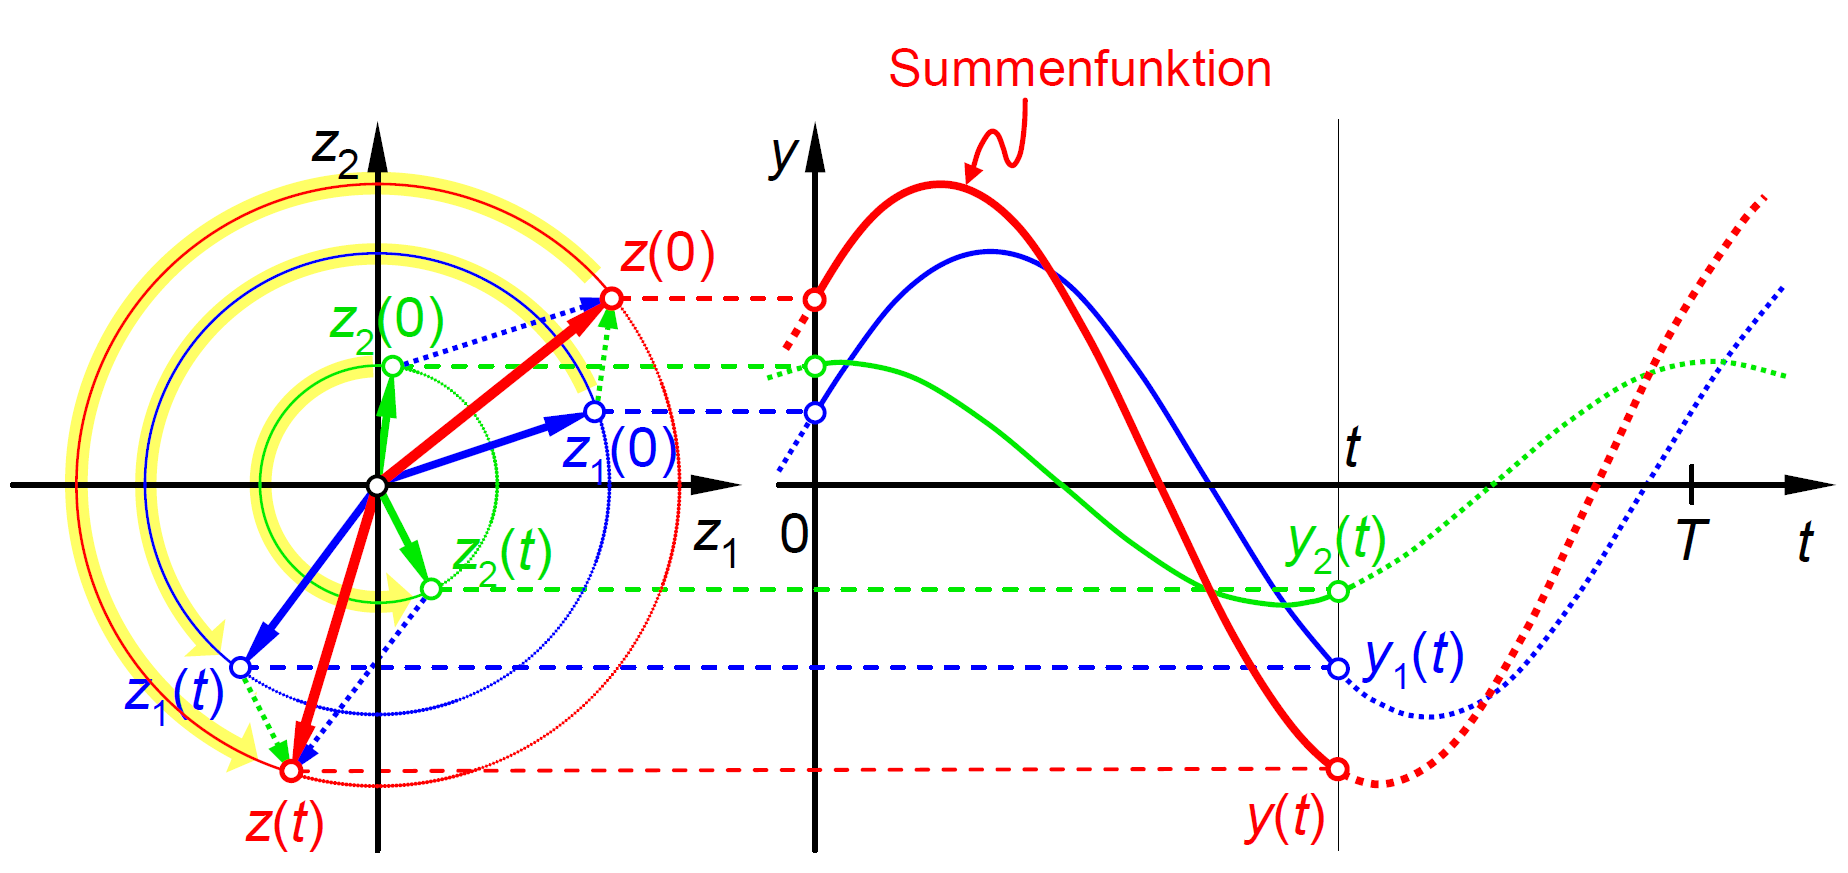
\includegraphics[width=\columnwidth]{images/summe-schwingungen.PNG}

\smallskip

\begin{tabular}{lll@{}}
    Komplexe Amplitude $z_i(0)$ & $z_i(0) = A \cdot \e^{\jimg \varphi_i}$                                                                                       & (zeitunabhängig)  \\
    'Schwingung' / 'Rotation'   & $z(t) = A \cdot \e^{\jimg (\omega t + \varphi)} = \underbrace{A \cdot \e^{\jimg \varphi}}_{z_i(0)} \cdot \e^{\jimg \omega t}$ & (zeitabhängig)
\end{tabular}


\para{Überlagerung gleichfrequenter Schwingungen ($\bm{z(t) = z_1(t) + z_2(t)}$)}
\begin{itemize}
    \item Überlagerung gleichfrequenter Schwingungen entspricht grafischer Addition der
    beiden 'Zeiger' zu jedem Zeitpunkt.
    \item La somma va eseguita solamente usando $\sin \text{o} \cos$, scegliere uno dei
    2 e trasformare l'altro usando prorietà trigonometriche (\ref{chap:trigo-beziehungen})
    \item Per trovare $A$: exp $\rightarrow$ kartesische, eseguire $\sum$, risultato da kartesiche $\rightarrow$ exp
\end{itemize}



\smallskip

\renewcommand{\arraystretch}{1.3}
\begin{tabular}{lll}
    reelle \cor{Amplitude}:   & $A = \vert A_1 \cdot \e^{\jimg \varphi_1} + A_2 \cdot \e^{\jimg \varphi_2} \vert =\cor{a} \cdot e^{\jimg\alpha}$      & (Betrag)  \\
    \cbl{Nullphasenwinkel}    & $\varphi_0 = \arg(A_1 \cdot \e^{\jimg \varphi_1} + A_2 \cdot \e^{\jimg \varphi_2}) =a \cdot e^{\jimg\cbl{\mathbf{\alpha}}}$   & (Winkel)	
\end{tabular}
\renewcommand{\arraystretch}{1}
        \section{Komplexe Funktionen (Abbildungen)}

\vspace{-0.2cm}

$$ f: \: \mathbb{D}_f \subseteqq \mathbb{C}  \: \rightarrow \: \mathbb{W}_f \subseteqq  \mathbb{C}, \: z  \mapsto w = f(z) $$

\begin{itemize}[itemsep=0.2cm]
    \item Winkeltreue für komplex differenzierbare Funktion mit $f'(z) \neq 0$ \\
        \textrightarrow\ Drehstreckung mit Drehwinkel $\arg[f'(z)]$ und Streckfaktor $\vert f'(z) \vert$\\
        \textrightarrow\ Winkelterue singifica che l'angolo di incidenza tra rette viene mantenuto
    \item Die Ableitung $f'(z)$ beschreibt, was lokal im Punkt $z$ passiert \\
        \textrightarrow\ Streckfaktor und Drehwinkel im Punkt $z$ \\
        Beispiel: $f'(z) = \frac{1}{2}\jimg$ \quad \textrightarrow\ Steckung um $\frac{1}{2}$ und Drehwinkel $\frac{\pi}{2}$
\end{itemize}

   

\subsubsection{Parametergleichung von Bildkurven}

Parametergleichung einer Bildgeraden kann \textbf{immer} ermittelt werden!

\smallskip

\begin{tabular}{ll}
    waagerechte Gerade: & $z = z(r) = r + \jimg c_2$ \quad mit $r \in \mathbb{R}$ \\
    senkrechte Gerade:  & $z = z(s) = c_1 + \jimg s$ \quad mit $r \in \mathbb{R}$
\end{tabular}\vspace{1em}

\begin{itemize}
    \item $c_1$ è lo Stützvektor sull'asse reale, $j$ è la direzione verticale.
    \item $j c_2$ è lo Stützvektor sull'asse immaginario, $1$ è la direzione orizzontale.
\end{itemize}

\smallskip

\textrightarrow\ in $w = f(z) $ so einsetzen und ausrechnen / vereinfachen \\
\textrightarrow\ Beispiel-Resultat:  $w = (r^2 - c^2) + \jimg 2 r c$


\subsubsection{Koordinatengleichung von Bildkurven}
\begin{enumerate}
    \item Separare parte Reale ed Immaginaria ($w_1 = \RE(w), w_2 = \IM(w)$)
    \item Sistema di equazioni e rimuovere parametri $r, s$
\end{enumerate}


\example{Kapitel \ref{chap:bsp_gitternetz}}

\columnbreak


\subsection{Lineare Funktion}

\vspace{-0.2cm}

$$ f: \: z \mapsto w = f(z) = az + b \quad \text{mit } a, \, b \in \mathbb{C} \text{ und } a \neq 0 $$

\begin{itemize}[itemsep=0.1cm]
    \item für $a = 1$ eine Translation um den Ortsvektor $\vec{b}$
    \item für $a \neq 1$ eine Drehstreckung mit Zentrum $\frac{b}{1-a}$, dem Drehwinkel $\arg(a)$ und dem Streckfaktor $\vert a \vert$
    \item Si può anche pensare come $a$: Streckung und drehung attorno ad $O$, $b$ verschiebung
\end{itemize}

\vspace{-0.1cm}

\begin{center}
    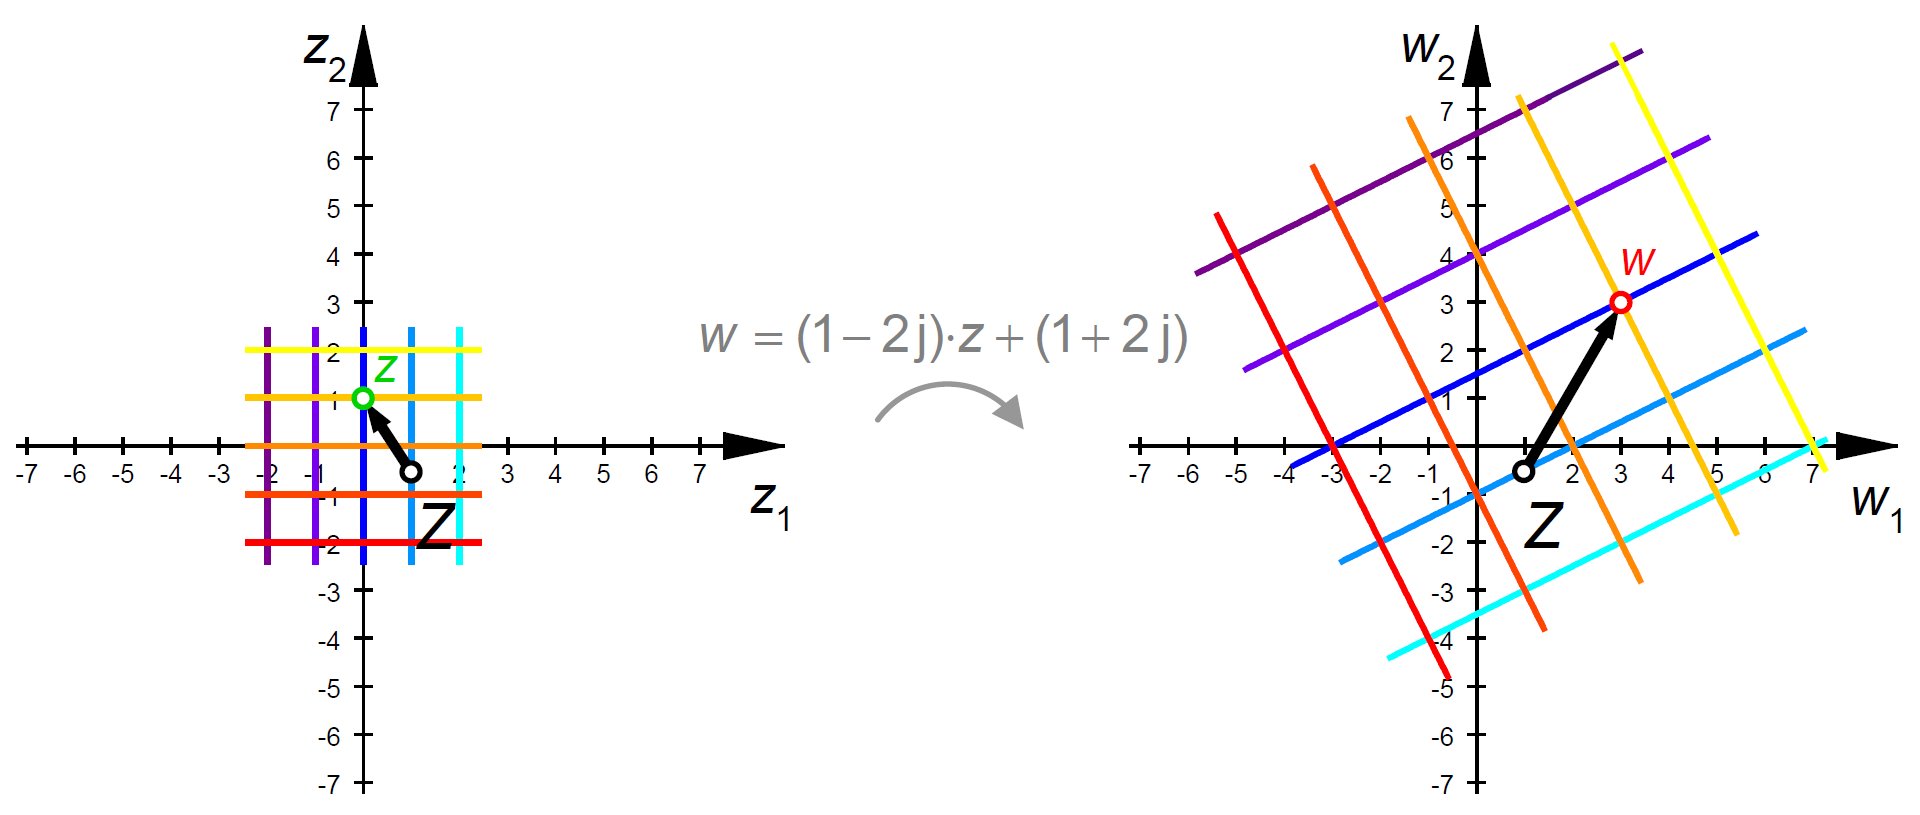
\includegraphics[width=0.85\linewidth]{images/lineare_abbildung.png}
\end{center}

\vspace{-0.1cm}


\subsection{Quadratfunktion / Wurzelfunktion}

\begin{tabular}{ll}
    $\bm{f(z) = z^2}$       & Verdoppelung des Winkels $\arg(z)$ und Quadrierung des \\  \medskip
                            & Abstandes zum Ursprung $\vert z \vert ^2$ \\
    $\bm{f(z) = \sqrt{w}}$  & Halbierung des Winkels $\arg(z)$ und (relle) Wurzel des Abstandes \\
                            & zum Ursprung $\vert z \vert$
\end{tabular}

\medskip


\para{Quadratfunktion (kartesische Koordinaten)}

\begin{center}
     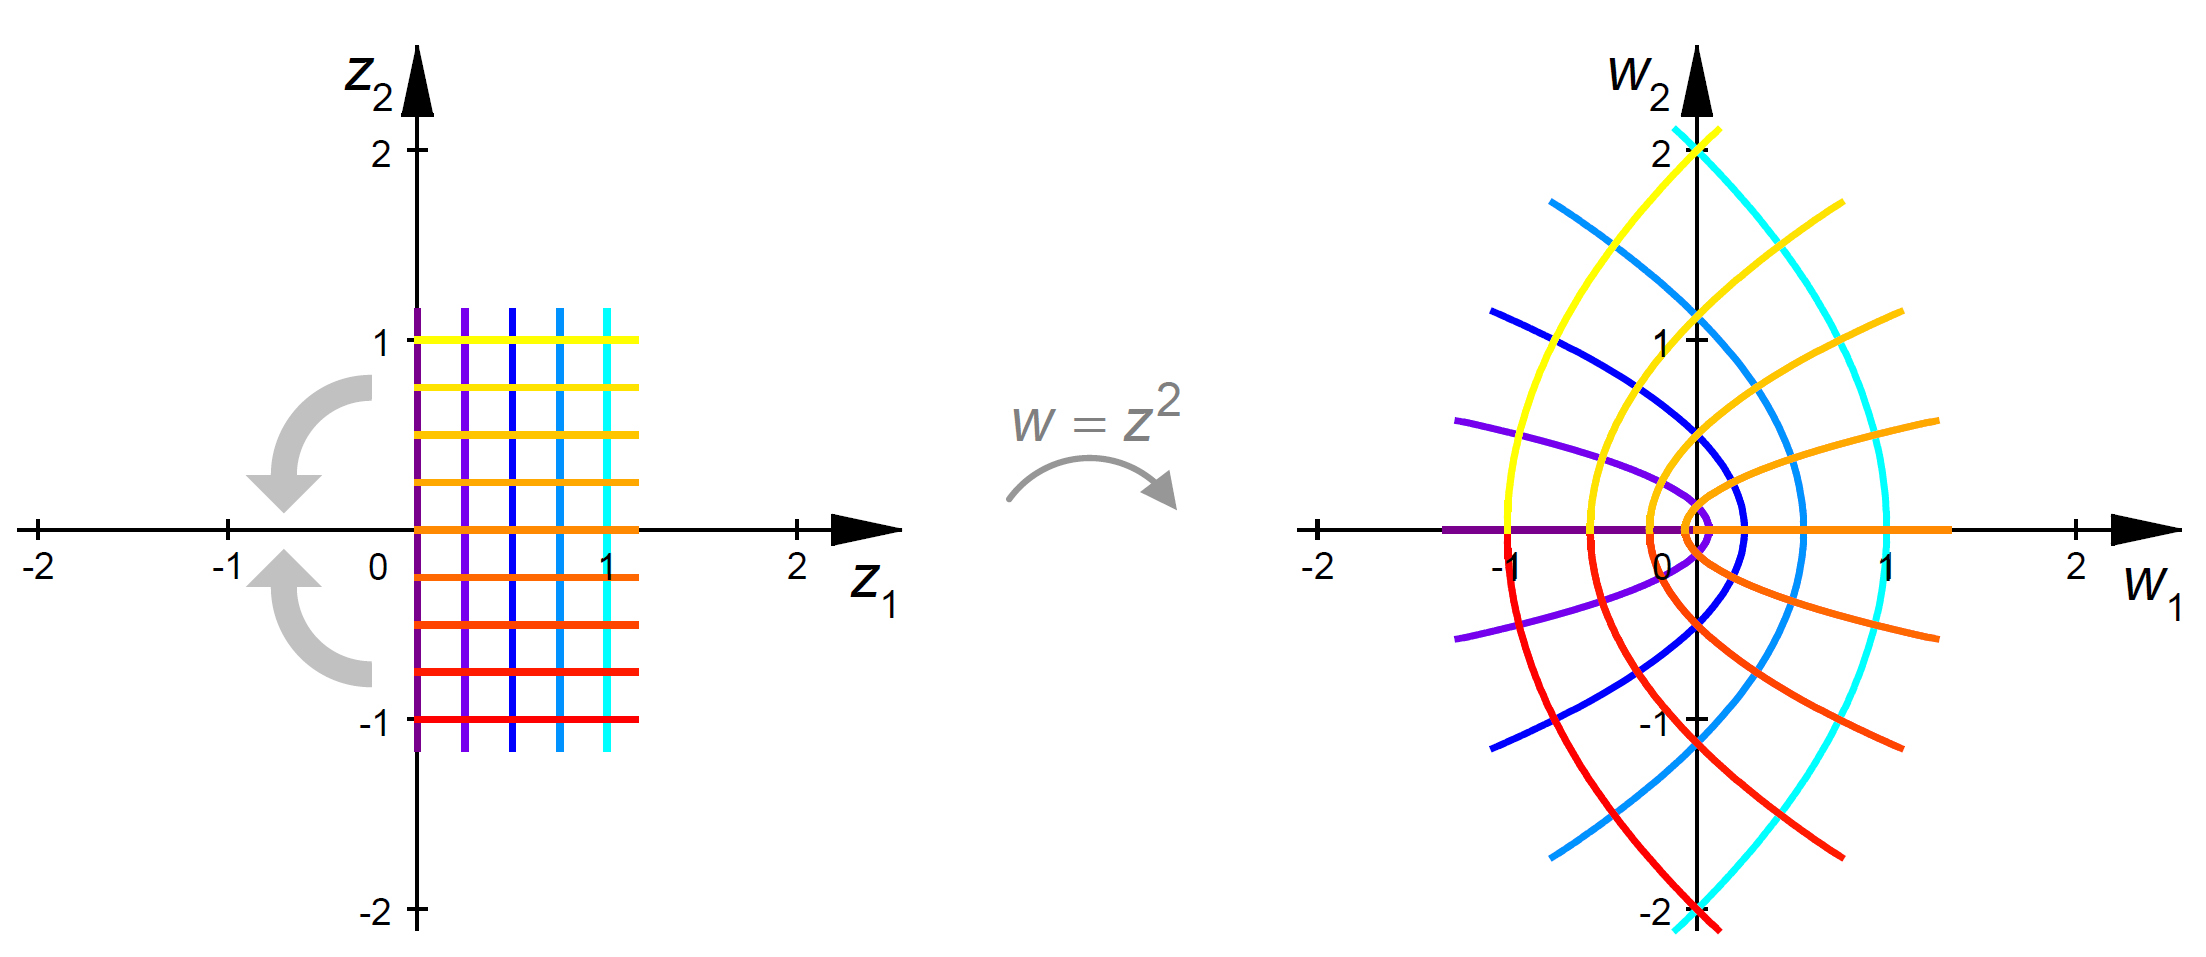
\includegraphics[width=0.85\linewidth]{images/quadratische_abbildung.PNG}
\end{center}
   
\vspace{-0.2cm}


\para{Quadratfunktion / Wurzelfunktion (Polarkoordinaten)}

\begin{center}
    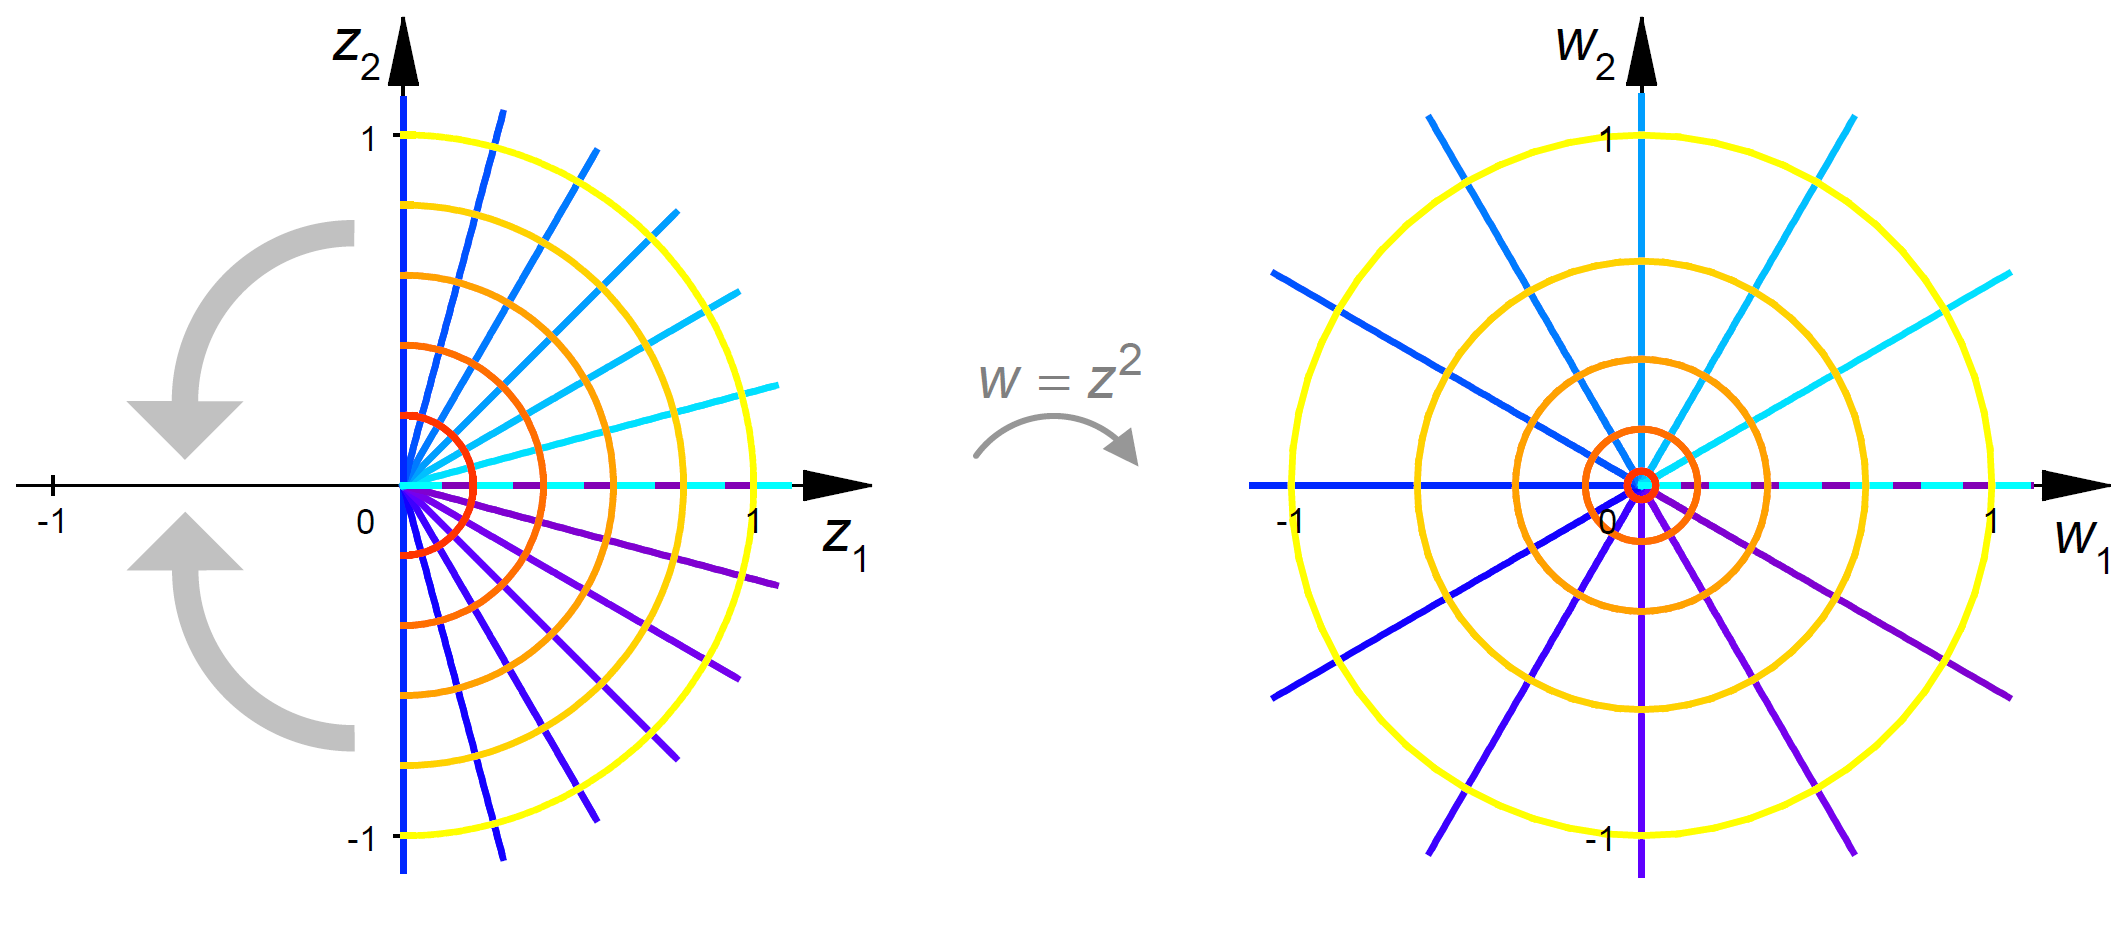
\includegraphics[width=0.85\linewidth]{images/quadratische_abbildung_2.PNG}
\end{center}

\vspace{-0.2cm}


\subsubsection{Eigenschaften der Quadrat- und Wurzelfunktion}

\begin{itemize}
    \item rechte Hälfte der $z$-Ebene wird schon auf ganze $w$-Ebene abgebildet
    \item Doppelwertig, wenn linke Hälfte auch noch abgebildet wird
    \item bijektiv, bei 2-blättriger Riemann'scher Fläche
    \item Quadratfunktion überall winkeltreu ausser im Ursprung, weil dort $f'(z) = 2 z = 0$
    \item Wurzelfunktion überall winkeltreu ausser im Ursprung, weil $f'(z) = \frac{1}{2 \sqrt{z}}$ nicht definiert
\end{itemize}


\subsection{Potenzfunktion / Wurzelfunktion} 

\begin{tabular}{ll}
    \medskip
    $\bm{f(z) = z^n}$           & $n$-facher Winkel von $\arg(z)$ und Abstand $\vert z \vert ^n$ zum Ursprung \\ 
    $\bm{f(z) = \sqrt[n]{w}}$   & $n$-ter Teil des Winkels $\arg(z)$ und (relle) $n$-te Wurzel des \\
                                & Abstandes zum Ursprung $\vert z \vert$ \\
\end{tabular}

\begin{center}
    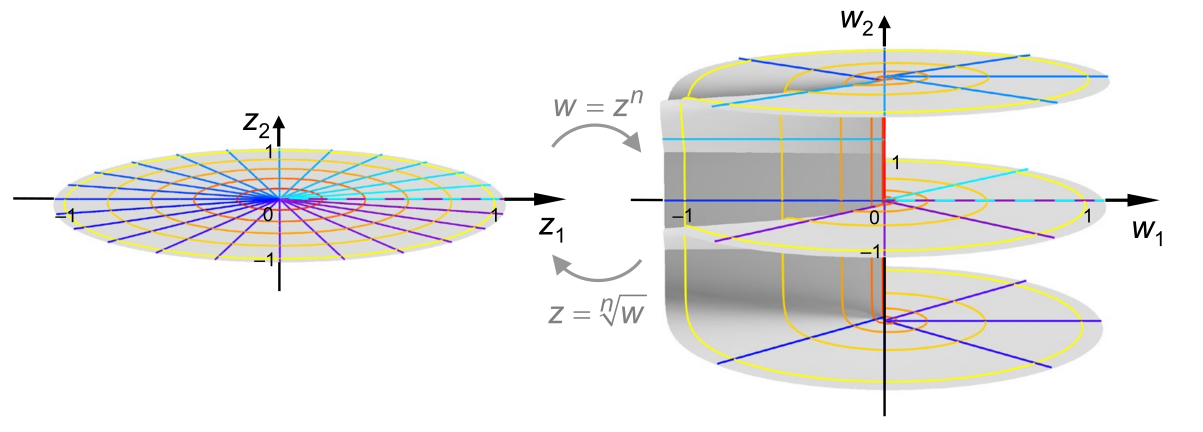
\includegraphics[width=0.8\columnwidth]{images/potenzfunktion.png}
\end{center}


\subsubsection{Eigenschaften der Potenz- und Wurzelfunktion}

\begin{itemize}
    \item bijektiv, bei $n$-blättriger Riemann'scher Fläche
    \item Beide Funktionen überall winkeltreu ausser im Ursprung
\end{itemize}


\subsection{Kreisspiegelung}\vspace{-1em}
\[f: \: z \mapsto w = \frac{1}{\overline{z}} \]

\begin{minipage}{0.64\columnwidth}    
    \setlength{\tabcolsep}{4pt}
    \begin{tabular}{llllll}
        Abstand: & $\vert w \vert = \frac{1}{\vert z \vert }$ & &  
        Winkel: & $\arg(w) = \arg(z)$
    \end{tabular}
    \setlength{\tabcolsep}{6pt}
    
    \subsubsection*{Eigenschaften der Kreisspiegelung}
    
    \begin{itemize}
        \item bijektiv auf $\mathbb{C} \: \cap \: \lbrace \infty \rbrace$
        \item winkeltreu (bis auf das Vorzeichen)
        \item Geraden / Kreise gehen in Geraden / Kreise über
        \item Einheitskreis ist ein \textbf{Fixpunktkreis}
        \item Rand eines Kreises geht in den Rand des Bildkreises über
    \end{itemize}
\end{minipage}
\begin{minipage}{0.36\columnwidth}
    \begin{center}
    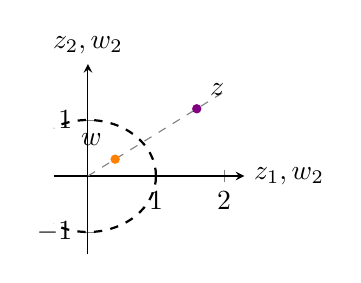
\begin{tikzpicture}
        [
            scale = 1.0,
            >=latex
        ]
        \begin{axis}[
            xmin=-0.5,
            xmax=2.3,
            ymin=-1.4,
            ymax=2,
            width=4cm,
            height=4cm,
            axis x line=middle, 
            axis y line=middle, 
            xtick={0, 1, 2},
            xticklabels={$0$, $1$, $2$},
            ytick={-1, 0, 1},
            x label style={anchor=west},
            xlabel={$\cvt{z_1}, \cor{w_2}$}, 
            y label style={anchor=south},
            ylabel={$\cvt{z_2}, \cor{w_2}$}
        ]
        
        % Cerchio unitario di riferimento
        \draw[black, thick, dashed] (axis cs:0,0) circle [radius=1];
        
        % Retta d'azione
        \addplot[gray, dashed, thin, domain=0:2] {0.75*x};
        
        % Punto z (|z| = 2)
        \node[circle, fill=violet, inner sep=1.2pt, label={above right:$z$}] at (axis cs:1.6, 1.2) {};
        
        % Punto w (immagine di z, |w| = 0.5)
        \node[circle, fill=orange, inner sep=1.2pt, label={above left:$w$}] at (axis cs:0.4, 0.3) {};

        \end{axis}
    \end{tikzpicture}
\end{center}
\end{minipage}

\subsubsection*{Vorgehen Bildkurve / Bildfläche zeichnen}

\begin{minipage}[t]{0.55\linewidth}
    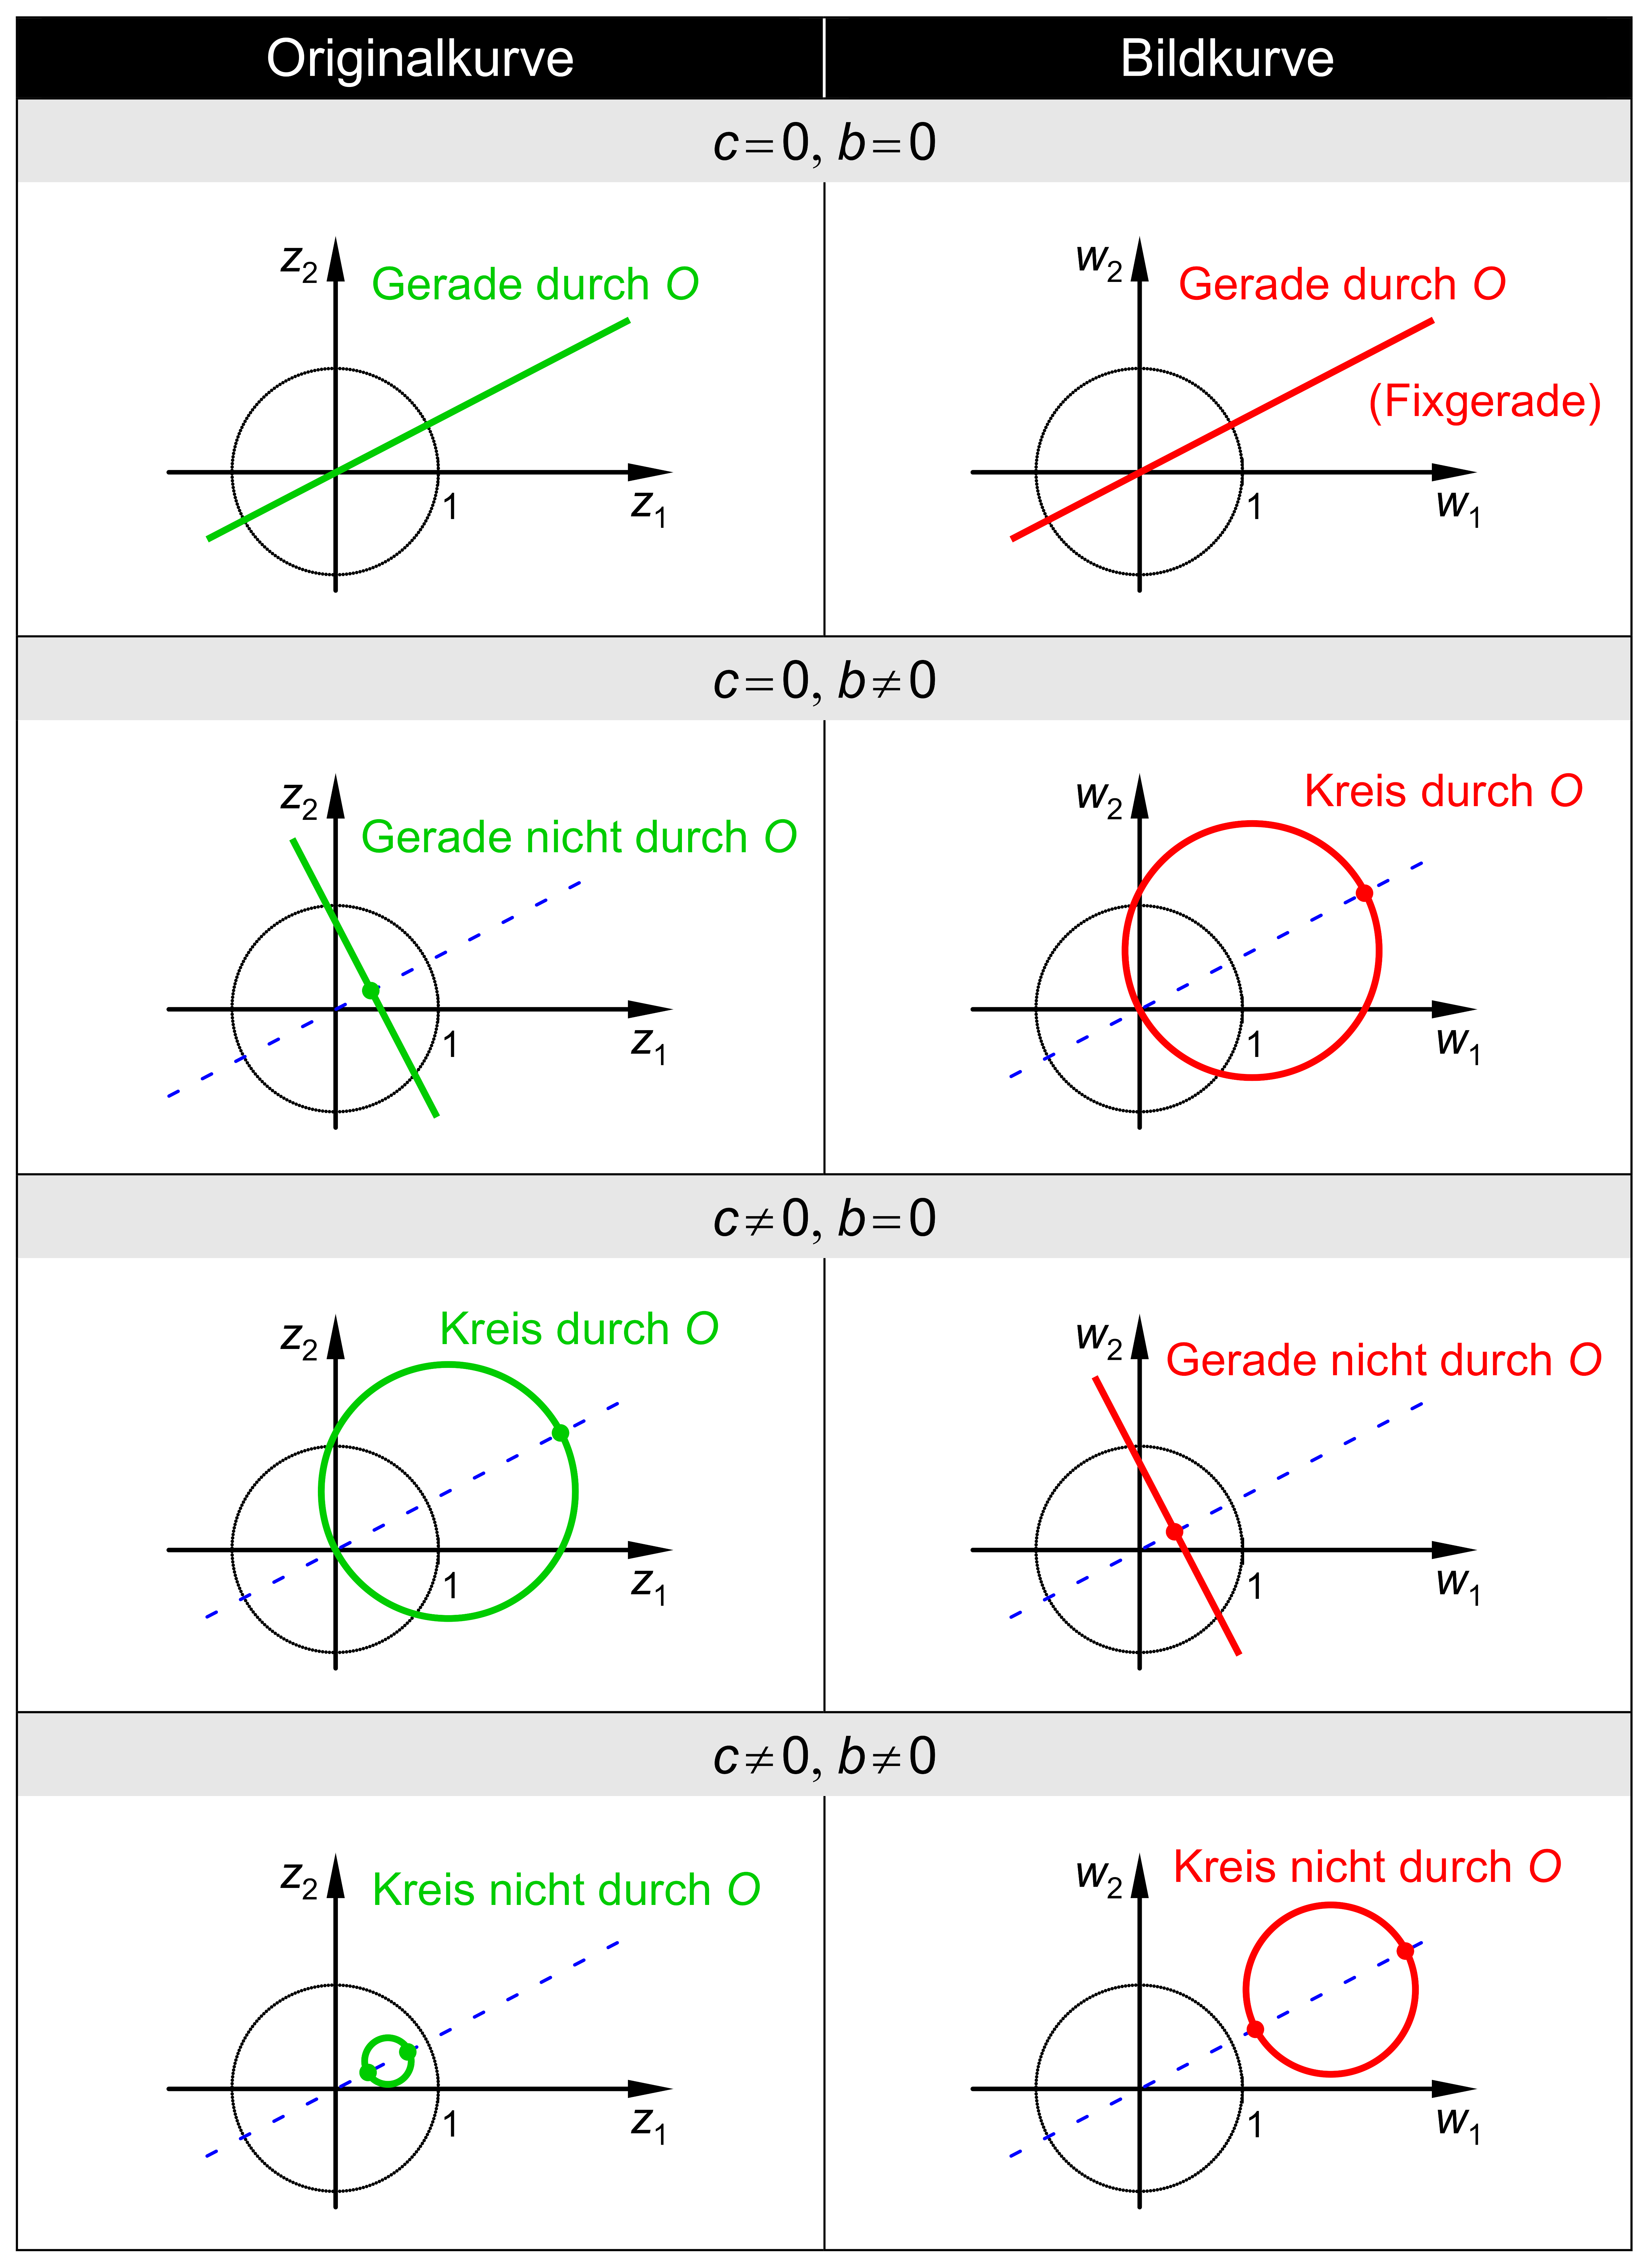
\includegraphics[width=\linewidth, align=t]{images/kreisspiegelung.png}
\end{minipage}
\hfill
\begin{minipage}[t]{0.43\linewidth}
    \raggedright

    \begin{enumerate}[itemsep=0.2cm]
        \item Ist  Bild eine Gerade oder ein Kreis?
        \item Gibt es Fixpunkte? (Einheitskreis)
        \item Abstand zu Ursprung auf Strahl reziprok
        \item Symmetrien beachten
        \item Fläche schraffieren: geeigneten Punkt aus Originalfläche abbilden
    \end{enumerate}

    \medskip

    \textbf{\color{red}Hinweis:} Bei Bedarf Originalkurve in Kreise und Geraden zerlegen\vspace{1em}!
    
    \textbf{Ortogonalità e Test Point}
    \begin{itemize}
        \item \textbf{Fixkreise (Cerchi fissi):} Un cerchio che interseca il cerchio unitario ortogonalmente ($90^\circ$) viene mappato su se stesso.
    \end{itemize}
\end{minipage}

\begin{itemize}
    \item \textbf{Test Point:} Per determinare l'area da colorare, usare un test point.
    \item \textbf{Segno di Im:} Con $1/z$ (reciproco), la parte immaginaria cambia segno; con $1/\bar{z}$ (inversione), il segno rimane invariato.
\end{itemize}

\columnbreak


\subsection{Kehrwertfunktion}

\vspace{-0.2cm}

$$ f: \: z \mapsto w = \frac{1}{z} $$

\begin{tabular}{lllllll}
    Abstand: & $\vert w \vert = \frac{1}{\vert z \vert }$ &  & & Winkel: & $\arg(w) = - \arg(z)$
\end{tabular}

\smallskip

\textbf{ \textrightarrow\ Grosse Ähnlichkeit zur Kreisspiegelung!}

% NOTE: Anregung / Idee für die Grafiken von Fabian Steiner
\begin{minipage}[c]{0.41\columnwidth}
    \begin{center}
    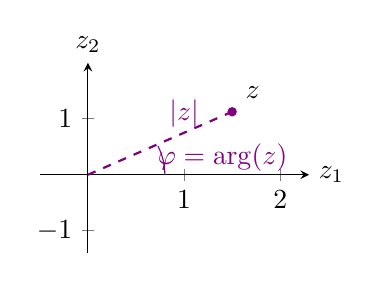
\begin{tikzpicture}
        [
            scale = 1.0,
            >=latex
        ]
        \begin{axis}[
            xmin=-0.5,
            xmax=2.3,
            ymin=-1.4,
            ymax=2,
            width=5cm,
            height=4cm,
            axis x line=middle, 
            axis y line=middle, 
            xtick={0, 1, 2},
            xticklabels={$0$, $1$, $2$},
            ytick={-1, 0, 1},
            x label style={anchor=west},
            xlabel={$z_1$}, 
            y label style={anchor=south},
            ylabel={$z_2$}
        ]
        
        \addplot[violet, dashed, thick, domain=0:1.5] {0.75*x};
        \draw[violet] (0.8, 0) arc[start angle=0, end angle=27, radius=0.8cm];
        \node[violet] at (1.4, 0.3) {$\varphi = \arg(z)$};
        
        \node[violet] at (1, 1.1) {$|z|$};

        \node[circle, fill=violet, inner sep=1.2pt, label={above right:$z$}] at (axis cs:1.5, 1.125) {};


        \end{axis}
    \end{tikzpicture}
\end{center}
\end{minipage}
\hfill
\begin{minipage}[c]{0.08\columnwidth}
    $$ \underrightarrow{w = \frac{1}{z}} $$
\end{minipage}
\hfill
\begin{minipage}[c]{0.41\columnwidth}
    \begin{center}
    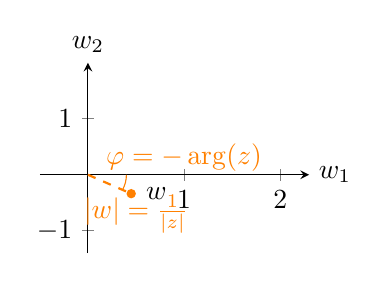
\begin{tikzpicture}
        [
            scale = 1.0,
            >=latex
        ]
        \begin{axis}[
            xmin=-0.5,
            xmax=2.3,
            ymin=-1.4,
            ymax=2,
            width=5cm,
            height=4cm,
            axis x line=middle, 
            axis y line=middle, 
            xtick={0, 1, 2},
            xticklabels={$0$, $1$, $2$},
            ytick={-1, 0, 1},
            x label style={anchor=west},
            xlabel={$w_1$}, 
            y label style={anchor=south},
            ylabel={$w_2$}
        ]
        
        \addplot[orange, thick,dashed, domain=0:0.45] {-0.75*x};
        \draw[orange] (0.4, 0) arc[start angle=0, end angle=-28, radius=0.4cm];
        \node[orange] at (1, 0.3) {$\varphi = -\arg(z)$};
        
        \node[orange] at (0.5, -0.7) {$|w| = \frac{1}{|z|}$};

        \node[circle, fill=orange, inner sep=1.2pt, label={right:$w$}] at (axis cs:0.45, -0.3375) {};

        \end{axis}
    \end{tikzpicture}
\end{center}
\end{minipage}


\subsection{Exponentialfunktion / Logarithmusfunktion}

\vspace{-0.2cm}

$$ \e^z = \e^{z_1} \cdot \e^{\jimg z_2} = \e^{z_1} \cjs(z_2) \qquad \qquad  
\Ln(z) = \ln(\vert z \vert) + \jimg \arg(z) $$

\textrightarrow\ Der Nullpunkt (Ursprung) wird \textbf{nicht} abgebildet!

\begin{center}
    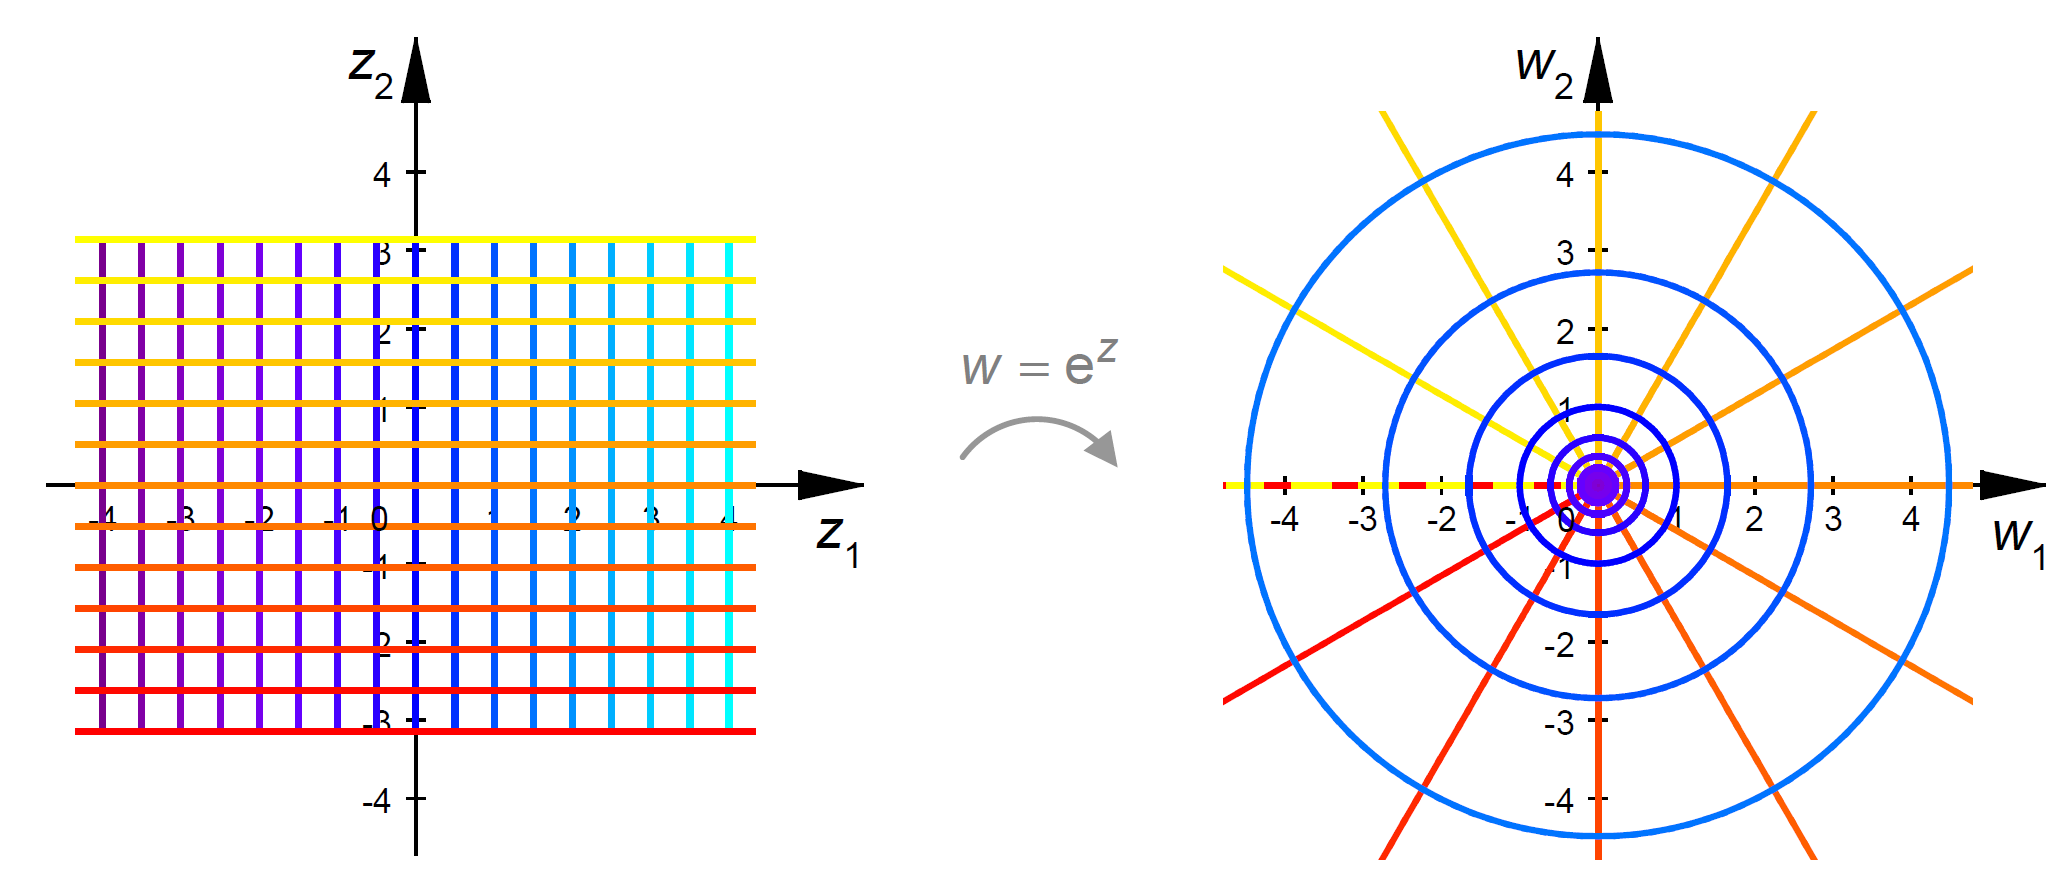
\includegraphics[width=0.85\linewidth]{images/exponentialfunktion.PNG}
\end{center}

\begin{itemize}
    \item Horizontale Geraden: Stahlen von Ursprung weg
    \item Vertikale Geraden: Kreise um Ursprung
\end{itemize}


\subsubsection{Eigenschaften der Exponential- und Logarithmusfunktion}

\begin{itemize}
    \item bijektiv, bei $\infty$-blättriger Riemann'scher Fläche ($2 \pi \jimg$-periodisch) ausser im Punkt $0$ (weil $\e^z \neq 0$)
    \item Exponentialfunktion $\e^z$ überall winkeltreu
    \item Umkehrfunktion $\Ln(w)$ überall in $\mathbb{D}_f$ winkeltreu ($\mathbb{C} \: \diagdown \; \lbrace 0 \rbrace$)
\end{itemize}


% Die Möbiustransformation ist Inhalt von Fabin Steiner 
% reformatting: Simone Stitz
\subsection{Möbisutransformation}

Die Möbiustransformation ist eine veralgemeinerung der Kehrwertsfunktion:
$$ f(z) = w = \frac{az + b}{cz + d} \qquad \qquad \text{Umkehrfunktion: } f(w) = z =\frac{-dw + b}{cw - a} $$
$a, \, b, \, c, \, d \in \mathbb{C}, \; c \neq0$ \& $ad - bc\neq 0$ \textrightarrow\ sonst wäre $f$ konstant


\smallskip

\resizebox{1\linewidth}{!}{%
\begin{circuitikz}
\tikzstyle{every node}=[font=\normalsize]
\draw [->, >=Stealth] (3.5,11.25) -- (6.5,11.25);
\node [font=\normalsize] at (4.75,11.5) {\textbf{$u=cz+d$}};
\node [font=\normalsize] at (5,11) {\textbf{lineare Funktion}};
\node [font=\normalsize] at (3,11.25) {\textbf{$f$: z}};
\draw [->, >=Stealth] (7.5,11.25) -- (10.5,11.25);
\node [font=\normalsize] at (8.75,11.5) {\textbf{$v=\frac{1}{u}$}};
\node [font=\normalsize] at (9,11) {\textbf{Kehrwertfunktion}};
\node [font=\normalsize] at (7,11.25) {\textbf{u}};
\draw [->, >=Stealth] (11.5,11.25) -- (14.5,11.25);
\node [font=\normalsize] at (12.75,11.5) {\textbf{$w=\frac{bc-ad}{c}v+\frac{a}{d}$}};
\node [font=\normalsize] at (13,11) {\textbf{lineare Funktion}};
\node [font=\normalsize] at (11,11.25) {\textbf{$v$}};
\node [font=\normalsize] at (14.75,11.25) {\textbf{w}};
\end{circuitikz}
}%


\subsubsection{Eigenschaften der Möbiustransformation}

\begin{itemize}
    \item Die Möbiustransformation ist winkel- und kreistreu
    \item Die Umkehrfunktion ist wieder eine Möbiustransformation \\
        \textbf{Achtung:} Es sind nur 3 Parameter! \textrightarrow\ ein Parameter kann gekürtzt werden
\end{itemize}

% Ende Code Fabian
        \section{Fourierreihen periodischer Funktionen}

Darstellung einer \textbf{periodischen} Funktion $f(t)$ mit Periodendauer $T > 0$ durch eine Linearkombination von Sinus- und Kosinusfunktionen,
deren Frequenzen ganzzahlige Vielfache der Kreisfrequenz (Winkelgeschwindigkeit) $\omega_f = \frac{2 \pi}{T} = 2 \pi v$ sind. 

\crd{\textbf{T periodish}: Endlich anzahl sprungstelle, $g- \in \infty$ und $g+ \in \infty$}

\smallskip

\textbf{Hinweis:} In \cbl{blau} ist jeweils die komplexe Fourier-Theorie abgebildet.
\[\FR[f(t)] = \frac{a_0}{2} + \sum\limits _{n=1}^\infty \big[ a_n \cdot \cos(n \, \omega_f \, t) + b_n \cdot \sin(n \, \omega_f \, t) \big] \]
\[\cbl{\FR[f(t)] = \sum\limits _{k = -\infty}^\infty \: \big( c_k \cdot \e^{\jimg \, k \, \omega_f \, t} \big)} \]


\subsection{Orthagonalitätsbeziehungen Basisfunktionen}

\begin{tabular}{ll}
    $\int \limits_{0}^{T} \cos(m \, \omega_f \, t) \cdot \cos(n \, \omega_f \, t) \, \diff t = 
    \begin{cases}
        T,              & m = n = 0 \\
        \frac{T}{2},    & m = n > 0 \\
        0,              & m \neq n
    \end{cases}$ 
    & $(m, \; n \in \mathbb{N}_0)$ \\
    \\
    $\int \limits_{0}^{T} \sin(m \, \omega_f \, t) \cdot \sin(n \, \omega_f \, t) \, \diff t =      		
    \begin{cases}
        \frac{T}{2},    & m = n     \\
        0,              & m \neq n
    \end{cases} $ 
    & $(m, \; n \in \mathbb{N})$    \\
    \\
    $\int \limits_{0}^{T} \cos(m \, \omega_f \, t) \cdot \sin(n \, \omega_f \, t) \, \diff t = 0$ 	
    & $(m \in \mathbb{N}_0, \; n \in \mathbb{N})$ 
\end{tabular}


\subsection{Berechnung der Fourier-Koeffizienten}

\textbf{$\bm{\frac{a_0}{2}}$ entspricht dem Mittelwert MWS (Gleichstromanteil) der Funktion
$\bm{f(t)}$\\auf dem Intervall [0 ; T)}

\renewcommand{\arraystretch}{2.5}
\begin{tabular}{l c l}
    % $a_0 = \frac{2}{T} \cdot \int \limits_{0}^{T} f(t) \, \diff t$\\
    $a_n = \frac{2}{T} \cdot \int \limits_{0}^{T} f(t) \cdot \cos(n \, \omega_f \, t) \, \diff t$                           & $(n = 0, \, 1, \, 2, \, \ldots)$                                                                  \\
    $b_n = \frac{2}{T} \cdot \int \limits_{0}^{T} f(t) \cdot \sin(n \, \omega_f \, t) \, \diff t$                           & $(n = 1, \, 2, \, 3, \, \ldots)$                                                                  \\	
    \cbl{$c_n = \overline{c_{-n}} = \frac{1}{T} \int \limits_0^T f(t) \cdot \e^{- \jimg \, n \, \omega_f \, t} \, \diff t$} & $\cbl{(n = 0, \, 1, \, 2, \, \ldots)}$    & \textrightarrow\ Für $n = 0: \, c_0 = \frac{a_0}{2}$
\end{tabular}
\renewcommand{\arraystretch}{1}

\smallskip

\begin{itemize}
    \item \crd{Trigo-Produkte in Integralen in SUMMEN umwandeln!!}
    \item \cor{Attenzione ad edge-cases con $n$ nei denominatori! (calcolare $n$ specifico
    separatemente con formula base)}
    \item \textbf{Integrazione a tratti:} dividere l'intervallo [0,T] in sotto-intervalli se 
    l'espressione analitica di $f(t)$ cambia nel periodo.
\end{itemize}
\subsubsection{Umrechnung der Fourierkoeffizienten}

\renewcommand{\arraystretch}{1.4}
\begin{tabular}{ll}
    $c_n = \overline{c_{-n}} = \frac{a_n - \jimg \, b_n }{2}$   & ($n = 0, \, 1, \, 2, \, \ldots \text{ wobei } b_0 = 0$)   \\
    $a_n = 2 \, \RE(c_n) = c_n + c_{-n}$                        & ($n = 0, \, 1, \, 2, \, \ldots$)                          \\
    $b_n = -2 \, \IM(c_n) = \jimg (c_n - c_{-n})$               & ($n = 1, \, 2, \, 3, \, \ldots$) 
\end{tabular}
\renewcommand{\arraystretch}{1}

\columnbreak


\subsection{Sätze zur Berechnung der Koeffizienten}

\subsubsection{Symmetrie von Funktionen}

\begin{minipage}{0.48\linewidth}
    \begin{tabular}{l | c | c}
                    & gerade    & ungerade  \\ 
        \hline
        gerade      & gerade    & ungerade  \\
        \hline
        ungerade    & ungerade  & gerade    \\
    \end{tabular}
\end{minipage}
\hfill
\begin{minipage}{0.43\linewidth}
    \begin{tabular}{ll}
        gerade:     &  $f(-t) = f(t)$ \\
        \\ 
        ungerade:   & $f(-t) = - f(t)$ 
    \end{tabular}
\end{minipage}

\smallskip
\renewcommand{\arraystretch}{2}
\begin{tabular}{l|l|l}
\textbf{Proprietà} & \multicolumn{2}{l}{\textbf{Coefficienti di Fourier}} \\ \hline
\multirow{2}{*}{$f(t)$ gerade}   & $\displaystyle a_n = \frac{4}{T} \int_{0}^{\frac{T}{2}} f(t) \cos(n \omega_f t) dt$ & $b_n = 0$ \\
                                 & \color{blue}{$\text{Im}(c_k) = 0$} & \color{blue}{$c_n = \frac{a_n}{2}$ (reell)} \\ \hline
\multirow{2}{*}{$f(t)$ ungerade} & $\displaystyle a_n = 0$ & $\displaystyle b_n = \frac{4}{T} \int_{0}^{\frac{T}{2}} f(t) \sin(n \omega_f t) dt$ \\
                                 & \color{blue}{$\text{Re}(c_k) = 0$} & \color{blue}{$c_n = j \frac{b_n}{2}$ (imaginär)} \\ \hline
\end{tabular}
\renewcommand{\arraystretch}{1}

\subsubsection{Linearität}
\begin{center}
    \crd{$f(t) \text{ und } g(t)$ mussen das gleiche periode $T$ haben.}
\end{center}

$f(x)$ mit Koeffizienten $a_n^{(f)} , \, b_n^{(f)}$ \qquad $g(x)$ mit Koeffizienten $a_n^{(g)} , \, b_n^{(g)}$ \\
\textrightarrow\ $h(t) = r \cdot f(t) + s \cdot g(t)$ mit festem $s, \, r \in \mathbb{R}$

$$ a_n^{(h)} = r \cdot a_n^{(f)} + s \cdot a_n^{(g)} \qquad \qquad b_n^{(h)} = r \cdot b_n^{(f)} + s \cdot b_n^{(g)} $$


\subsubsection{Zeitstreckung / -stauchung / -spiegelung ("Ähnlichkeit")}

$g(t) = f(r \cdot t)$ mit $0 \neq r \in \mathbb{R}$ \qquad \cor{$\omega_g = \frac{2 \pi}{T_g}$ in Basisfunktionen!}

$$ a_n^{(g)} = a_n^{(f)} \qquad \qquad b_n^{(g)} = \sgn(r) \cdot b_n^{(f)} $$


\subsubsection{Zeitverschiebung}
$g(t) = f(t + t_0)$

\smallskip

\renewcommand{\arraystretch}{1.7}
\begin{tabular}{ll}
    $ a_n^{(g)} = \cos(n \, \omega_f \, t_0) \cdot a_n^{(f)} + \sin(n \, \omega_f \, t_0) \cdot b_n^{(f)}$      & $n = 0$ \quad [mit $b_0 = 0, \, 1, \, 2, \, \ldots$]  \\ 
    $ b_n^{(g)} = -\sin(n \, \omega_f \, t_0) \cdot a_n^{(f)} + \cos(n \, \omega_f \, t_0) \cdot  b_n^{(f)}$    & $n = 1, \, 2, \, 3, \, \ldots$                        \\	
    $ \cbl{c_k^{(g)} = \e^{\jimg \, k \, \omega_f \, t_0} \cdot c_k^{(f)}}$                                     & $\cbl{k  =1, \, 2, \, 3, \, \ldots}$
\end{tabular}
\renewcommand{\arraystretch}{1}


\subsection{Konvergenzverhalten von Fourierreihen}

\subsubsection{Optimalität der Fourierreihe}

Abstand zwischen zwei Funktionen zeigt, wie gut die Approximation der Funktion ist \\
\textrightarrow\ $f$ und $g$ sind $T$-periodisch und stückweise stetig mit Limes

$$ \Vert f - g \Vert = \sqrt{\frac{2}{T} \int \limits_0^T  [f(t) - g(t)]^2 \, \diff t } $$ 

\textrightarrow\ Fourier-Reihe approximiert eine Funktion am Besten!

\smallskip

mittlere quadrierte Abweichung: $\frac{T}{2} \vert \vert f - g \vert \vert ^2$


\subsubsection{Bessel'sche Ungleichung}

unendlich-dimensionaler Satz von Pythagoras
$$ \frac{a_0^2}{2} + \sum \limits_{n=1}^\infty \big( a_n^2 + b_n^2 \big) \leq  \frac{2}{T} \int \limits_0^T \big[f(t) \big]^2 \, \diff t = \Vert f \Vert ^2 $$


\subsubsection{Satz von Parseval}

unendlich-dimensionaler Satz von Pythagoras \textrightarrow\ Summe der Quadrate ist beschränkt
$$ \frac{a_0^2}{2} + \sum \limits_{n=1}^\infty \big( a_n^2 + b_n^2 \big) = \frac{2}{T} \int \limits_0^T [f(t)]^2 \, \diff t = \Vert f \Vert ^2 $$
$$ \cbl{ \sum \limits_{k= -\infty}^\infty \vert c_k \vert ^2 = \frac{1}{T} \int \limits_0^T \big[ f(t) \big]^2 \, \diff t } $$


\subsubsection{Konvergenz im Mittel}

Jede Funktion $f$ kann durch eine abbrechende Fourierreihe bezüglich ihres Abstandes beliebig genau approximiert werden.
Die Fläche zwischen Approximation und Funktion geht gegen 0 \quad $\Vert s_m(t) - f(t) \Vert \searrow 0$ \\
\textrightarrow\ Das heisst nicht, dass man überall absolute Übereinstimmung hat!

$$ \lim \limits_{m \to 0} \Vert \sum\limits _{n=1}^m \big[ a_n \cdot \cos(n \, \omega_f \, t) + b_n \cdot \sin(n \, \omega_f \, t) \big] - f(t) \Vert = 0 $$
$$ \cbl{\lim \limits_{m \to 0} \Vert \sum\limits _{k= -m}^m \: \big( c_k \, \e^{ \jimg \, k \, \omega_f \, t} \big) - f(t) \Vert = 0} $$


\subsubsection{Konvergenz der Fourierkoeffizienten}

Die Fourierkoeffizienten bilden Nullfolgen 

\renewcommand{\arraystretch}{2}
\begin{tabular}{l}
    $\lim \limits_{n \to \infty} a_n = \lim \limits_{n \to \infty} \frac{2}{T} \int \limits_0^T f(t) \cdot \cos(n\, \omega_f \, t) \, \diff t = 0$                                                                  \\
    $\lim \limits_{n \to \infty} b_n = \lim \limits_{n \to \infty} \frac{2}{T} \int \limits_0^T f(t) \cdot \sin(n\, \omega_f \, t) \, \diff t = 0$                                                                  \\
    $\cbl{\lim \limits_{n \to \infty} c_n = \lim \limits_{n \to \infty} \overline{c_{-n}} = \lim \limits_{n \to\infty} \frac{1}{T} \int \limits_0^T f(t) \cdot  \e^{- \jimg \, n \, \omega_f \, t} \, \diff t = 0}$
\end{tabular}
\renewcommand{\arraystretch}{1}


\subsubsection{Konvergenzgeschwindingkeit der Fourierkoeffizienten}

Ist die $T$-periodische Funktion $f$ ($m-2$)-mal stetig differenzierbar und ihre ($m-1$)-ste Ableitung stückweise stetig mit Limes und 
stückweise monoton, so existiert eine (nur von $f$ abhängige) Konstante $\in \mathbb{R}$ mit

$$ \vert a_n \vert \leq \frac{c}{n^m} \quad \text{und} \quad \vert b_n \vert \leq \frac{c}{n^m} \quad (m, \, n \in \mathbb{N}) $$


\subsubsection{Punktweise Konvergenz (Satz von Dirichlet)}

Wenn die linksseitige $f(t_0 - 0)$ \textbf{und} die rechtsseitige Ableitung $f(t_0 + 0)$ existieren, dann konvergiert die Fourierreihe gegen:	

$$ \frac{f(t_0 - 0) + f(t_0 + 0)}{2} \qquad \text{(Mitte einer Sprungstelle)} $$


Ist die Funktion in $t_0$ \textbf{stetig} und die beidseitigen Ableitungen existieren, dann konvergiert die Fourierreihe gegen:	

$$ \frac{f(t_0 - 0) + f(t_0 + 0)}{2} = \frac{f(t_0) + f(t_0)}{2} = f(t_0) \qquad \text{(Funktionswert)} $$

\textbf{Hinweis:}
Der Satz von Dirichlet wird gebraucht, um aus Fourier-Koeffizienten Reihen darzustellen. \\
\textbf{ \textrightarrow\ Passende Entwicklungsstelle $\bm{t_0}$ verwenden!}

\columnbreak

% Beginn Code Fabian Steiner (reformatted and slightly modified)
\subsection{Summenberechnung S mit Fourierreihe}

Die Summenberechnung soll anhand eines Beispiels erklärt werden.

\example{Summenberechnung mit Fourierreihe}

Aus der gegebenen Fourierreihe $\FR[\sin(t)]$ soll die Summe S berechnet werden:
$$ FR[\sin(t)] = \frac{1}{2\pi} + \frac{15}{5\pi} * \cos(t) + \frac{13}{2\pi} * \sin(t) + \frac{15}{7\pi} * \cos(t) + \ldots $$
$$ S = \frac{1}{5} + \frac{1}{7} + \frac{1}{9} + \ldots $$

In der Fourierreihe $\FR[\sin(t)]$ soll $t$ so gewählt werden, dass die Schwingungen wegfallen und die Koeffizienten möglichst der Summe ähneln. \\
\textrightarrow\ Wähle $t=0$, sodass übrig bleibt:

$$ \underbrace{\frac{1}{2\pi} + \frac{15}{5\pi} + \frac{15}{7\pi} + \ldots}_{Q} = \sin(0) = 0 $$

Dies entspricht noch nicht der gesuchten Summe $S$. Es ist eine \textbf{Umformung} nötig:
$$ Q * \frac{\pi}{15} = \frac{1}{30} + \underbrace{\frac{1}{5} + \frac{1}{7}+ \ldots}_{S} \qquad \underrightarrow{\text{auflösen nach }S} \qquad
\bm{S = -\frac{1}{30}} $$
% Ende Code Fabian Steiner


\subsection{Gibbs'sches Phänomen}

Fourierreihen überschwingen bei Sprungstellen um 8.94 \% 

\smallskip

\textrightarrow\ Je mehr Summanden in der Fourierreihe sind, desto kleiner ist der Effekt dieser Überschwinger! 

\begin{center}
    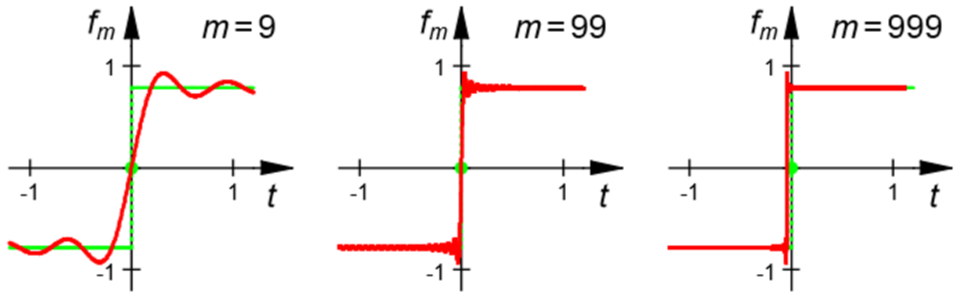
\includegraphics[width=0.85\linewidth]{images/gibbs.PNG}
\end{center}


        \input{sections/04_spektren.tex}
        \section{Sonstiges}
\subsection{Beispiel gitternetz}\label{chap:bsp_gitternetz}

La funzione mappa il piano $z$ nel piano $w = w_1 + j w_2$. Utilizzando la decomposizione $z = z_1 + j z_2$, la trasformazione è definita da:
\[ w = (z_1 + j z_2)^2 = (z_1^2 - z_2^2) + j(2 z_1 z_2) \]
Da cui le coordinate cartesiane nel piano $w$:
\[
\begin{cases}
    w_1 = z_1^2 - z_2^2 \\
    w_2 = 2 z_1 z_2
\end{cases}
\]

Ora, usando come argomento per $f$ le formule delle rette cartesiane, analizziamo la trasformazione

\begin{minipage}[t]{0.48\linewidth}
    \textbf{Verticali ($z = c_1 + js$):}
    Fissando la parte reale $z_1 = c_1$:
    \[ \begin{cases} w_1 = c_1^2 - s^2 \\ w_2 = 2c_1s \rightarrow s = \frac{w_2}{2c_1} \end{cases} \]
    Sostituendo $s$ in $w_1$:
    \[ \colorbox{blue!10}{$w_1 = c_1^2 - \frac{w_2^2}{4c_1^2}$} \]
    Rappresenta \textbf{parabole} con asse $w_1$ aperte a sinistra.
\end{minipage}
\hfill
\begin{minipage}[t]{0.48\linewidth}
    \textbf{Orizzontali ($z = r + jc_2$):}
    Fissando la parte immaginaria $z_2 = c_2$:
    \[ \begin{cases} w_1 = r^2 - c_2^2 \\ w_2 = 2rc_2 \rightarrow r = \frac{w_2}{2c_2} \end{cases} \]
    Sostituendo $r$ in $w_1$:
    \[ \colorbox{green!10}{$w_1 = \frac{w_2^2}{4c_2^2} - c_2^2$} \]
    Rappresenta \textbf{parabole} con asse $w_1$ aperte a destra.
\end{minipage}

\vspace{1.5em}

\subsubsection{Procedimento inverso}
\paragraph{Esempio: Griglia quadrata}
\[f(z) = z^2 \quad \rightarrow \quad f(z) = (z_1 + z_2 \jimg)^2 = z_1^2 + \jimg 2 z_1
z_2 - z_2^2\]
\[w_1 = \RE(w) = z_1^2 - z_2^2 \qquad w_2 = \IM(w) = 2z_1z_2\]
Ora sappiamo che in una griglia quadrata $w_1 / w_2$ sono costanti ($x,y$) quindi:\vspace{1em}

\begin{minipage}{0.45\columnwidth}
    \[z_1^2 - z_2^2 = c_1\]
    \begin{center}
        Iperbole orizzontale
    \end{center}
\end{minipage}\hfill
\begin{minipage}{0.45\columnwidth}
    \[c_2 = 2z_+z_2 \rightarrow z_2 = \frac{c_2}{2 z_1}\]
    \begin{center}
        Iperbole $x^-1$
    \end{center}
\end{minipage}

\subsection{Cambio indici}

L'obiettivo dell'ottimizzazione è eliminare i termini nulli della sommatoria ($\sum$) 

Per mappare una progressione aritmetica di indici che contenga solo i termini non nulli, si utilizza la relazione:
\[ n = (\text{passo} \cdot m) + \text{offset} \]
dove $m = 0, 1, 2, \dots$ è il nuovo indice di sottomatice (\textbf{m parte da 0!}). 

\begin{ctabular}{@{}lccccl@{}}
\toprule
\textbf{Target (n)} & \textbf{Passo} & \textbf{Offset} & \textbf{Formula} & \textbf{Esempio Sequenza} \\ \midrule
Dispari             & 2              & 1               & $n = 2m + 1$     & $1, 3, 5, 7, \dots$       \\
Pari                & 2              & 2               & $n = 2m + 2$     & $2, 4, 6, 8, \dots$       \\
Ogni 4 (da 1)       & 4              & 1               & $n = 4m + 1$     & $1, 5, 9, 13, \dots$      \\
Ogni 4 (da 3)       & 4              & 3               & $n = 4m + 3$     & $3, 7, 11, 15, \dots$     \\ \bottomrule
\end{ctabular}

\newpage
        \section{Mathematische Grundlagen}

\subsection{Trigonometrie}

\begingroup
\renewcommand{\arraystretch}{2}
\setlength{\tabcolsep}{0mm}
\scalebox{0.33}{
    \Huge
    \begin{tabularx}{3\columnwidth}{rp{1mm}V{3}*{17}{C}}
        \rowcolor{subsectioncolor!30}$\bm{\alpha}$\phantom{${}^{\circ}$} && $0$ & $\dfrac{\pi}{6\mathstrut}$ & $\dfrac{\pi}{4}$ & $\dfrac{\pi}{3}$ & $\dfrac{\pi}{2}$ & $\dfrac{2\pi}{3}$ & $\dfrac{3\pi}{4}$ & $\dfrac{5\pi}{6}$ & $\pi$ & $\dfrac{7\pi}{6}$ & $\dfrac{5\pi}{4}$ & $\dfrac{4\pi}{3}$ & $\dfrac{3\pi}{2}$ & $\dfrac{5\pi}{3}$ & $\dfrac{7\pi}{4}$ & $\dfrac{11\pi}{6}$ & $2\pi$ \\\hline
        \rowcolor{subsectioncolor!30}$\bm{\alpha^\circ}$ && \phantom{${}^\circ$}$0^\circ$ & $30^\circ$ & $45^\circ$ & $60^\circ$ & $90^\circ$ & $120^\circ$ & $135^\circ$ & $150^\circ$ & $180^\circ$ & $210^\circ$ & $225^\circ$ & $240^\circ$ & $270^\circ$ & $300^\circ$ & $315^\circ$ & $330^\circ$ & $360^\circ$ \\\hline
        $\bm{\sin(\alpha)}$ && $0$ & $\dfrac{1}{2\mathstrut}$ & $\dfrac{\sqrt{2}}{2}$ & $\dfrac{\sqrt{3}}{2}$ & $1$ & $\dfrac{\sqrt{3}}{2}$ & $\dfrac{\sqrt{2}}{2}$ & $\dfrac{1}{2}$ & $0$ & $-\dfrac{1}{2}$ & $-\dfrac{\sqrt{2}}{2}$ & $-\dfrac{\sqrt{3}}{2}$ & $-1$ & $-\dfrac{\sqrt{3}}{2}$ & $-\dfrac{\sqrt{2}}{2}$ & $-\dfrac{1}{2}$ & $0$ \\\hline
        $\bm{\cos(\alpha)}$ && $1$ & $\dfrac{\sqrt{3}}{2\mathstrut}$ & $\dfrac{\sqrt{2}}{2}$ & $\dfrac{1}{2}$ & $0$ & $-\dfrac{1}{2}$ & $-\dfrac{\sqrt{2}}{2}$ & $-\dfrac{\sqrt{3}}{2}$ & $-1$ & $-\dfrac{\sqrt{3}}{2}$ & $-\dfrac{\sqrt{2}}{2}$ & $-\dfrac{1}{2}$ & $0$ & $\dfrac{1}{2}$ & $\dfrac{\sqrt{2}}{2}$ & $\dfrac{\sqrt{3}}{2}$ & $1$ \\\hline
        $\bm{\tan(\alpha)}$ && $0$ & $\dfrac{\sqrt{3}}{3\mathstrut}$ & $1$ & $\sqrt{3}$ & $\pm\infty$ & $-\sqrt{3}$ & $-1$ & $-\dfrac{\sqrt{3}}{3}$ & $0$ & $\dfrac{\sqrt{3}}{3}$ & $1$ & $\sqrt{3}$ & $\pm\infty$ & $-\sqrt{3}$ & $-1$ & $-\dfrac{\sqrt{3}}{3}$ & $0$ \\\hline
        $\bm{\cot(\alpha)}$ && $\pm\infty$ & $\sqrt{3}$ & $1$ & $\dfrac{\sqrt{3}}{3\mathstrut}$ & $0$ & $-\dfrac{\sqrt{3}}{3}$ & $-1$ & $-\sqrt{3}$ & $\pm\infty$ & $\sqrt{3}$ & $1$ & $\dfrac{\sqrt{3}}{3}$ & $0$ & $-\dfrac{\sqrt{3}}{3}$ & $-1$ & $-\sqrt{3}$ & $\pm\infty$ \\
    \end{tabularx}}
\endgroup
    
\[\sin(\alpha) = \frac{\rm C. Opposto}{\rm Ipotenusa} \qquad \qquad \cos(\alpha) = \frac{\rm C. Adiacente}{\rm Ipotenusa}\]

\subsubsection{Beziehungen zwischen $\bm{\sin(x)}$ und $\bm{\cos(x)}$}\label{chap:trigo-beziehungen}

\renewcommand{\arraystretch}{1.2}
\begin{tabular}{ll}
    $\sin(-a) = -\sin(a)$                                                               & $\cos(-a) = \cos(a)$          \\
    $\sin(\pi - a) = \sin(a)$                                                           & $\cos(\pi -a) = - \cos(a)$    \\		
    $\sin(\pi + a) = -\sin(a)$                                                          & $\cos(\pi + a) = - \cos(a)$   \\	
    $\sin \Big( \frac{\pi}{2} - a \Big) = \sin \Big( \frac{\pi}{2} + a \Big) = \cos(a)$ & $\cos \Big( \frac{\pi}{2} - a \Big) = - \cos \Big( \frac{\pi}{2} + a \Big) = \sin(a)$		 
\end{tabular}
\renewcommand{\arraystretch}{1}


\subsubsection{Additionstheoreme}

\renewcommand{\arraystretch}{1.2}
\begin{tabular}{l}
    $\sin(a \pm b) = \sin(a) \cdot \cos(b) \pm \cos(a) \cdot \sin(b)$           \\
    $\cos(a \pm b) = \cos(a) \cdot \cos(b) \mp \sin(a) \cdot \sin(b) $          \\
    $\tan(a \pm b) = \frac{\tan(a) \pm \tan(b)}{1 \mp \tan(a) \cdot \tan(b)}$
\end{tabular}
\renewcommand{\arraystretch}{1}


\subsubsection{Summen und Differenzen}

\renewcommand{\arraystretch}{1.2}
\begin{tabular}{l}
    $\sin(a) + \sin(b) = 2 \cdot \sin \Big( \frac{a+b}{2} \Big) \cdot \cos \Big( \frac{a-b}{2} \Big)$   \\
    $\sin(a) - \sin(b) = 2 \cdot \sin \Big( \frac{a-b}{2} \Big) \cdot \cos \Big( \frac{a+b}{2} \Big)$   \\
    $\cos(a) + \cos(b) = 2 \cdot \cos \Big( \frac{a+b}{2} \Big) \cdot \cos \Big( \frac{a-b}{2} \Big)$   \\
    $\cos(a) - \cos(b) = -2 \cdot \sin \Big( \frac{a+b}{2} \Big) \cdot \sin \Big( \frac{a-b}{2} \Big)$  \\
    $\tan(a) \pm \tan(b) = \frac{\sin(a \pm b)}{\cos(a) \cdot \cos(b)}$ 
\end{tabular}
\renewcommand{\arraystretch}{1}


\subsubsection{Produkte}

\renewcommand{\arraystretch}{1.2}
\begin{tabular}{l}
    $\sin(a) \cdot \sin(b) = \frac{1}{2} \big( \cos(a-b) - \cos(a+b) \big) $ \\
    $\cos(a) \cdot \cos(b) = \frac{1}{2} \big( \cos(a-b) + \cos(a+b) \big) $ \\	
    $\sin(a) \cdot \cos(b) = \frac{1}{2} \big( \sin(a-b) + \sin(a+b) \big) $ 
\end{tabular}
\renewcommand{\arraystretch}{1}


\subsubsection{Winkelvielfache und Halbwinkel}

\renewcommand{\arraystretch}{1.2}
\begin{tabular}{l}
    $\sin(2a) = 2 \, \sin(a) \cdot \cos(a)$                                 \\
    $\sin(3a) = 3 \, \sin(a) -4 \, \sin^3(a)$                               \\ \medskip
    $\sin(4a) = 8 \, \cos^3(a) \cdot \sin(a) - 4 \, \cos(a) \cdot \sin(a)$  \\
    $\cos(2a) = \cos^2(a) - \sin^2(a)$                                      \\
    $\cos(3a) = 4 \, \cos^3(a) -3 \, \cos(a)$                               \\  \medskip 
    $\cos(4a) = 8 \, \cos^4(a) - 8 \, \cos^2(a) + 1$                        \\
    $\sin \Big( \frac{a}{2} \Big) = \sqrt{\frac{1}{2} \big(1-\cos(a) \big)} \qquad \cos \Big( \frac{a}{2} \Big) = \sqrt{\frac{1}{2} \big(1+\cos(a) \big)}$ 
\end{tabular}
\renewcommand{\arraystretch}{1}


\subsubsection{Potenzen}

\renewcommand{\arraystretch}{1.2}
\begin{tabular}{ll}
    $\sin^2(a) = \frac{1}{2} \big(1-\cos(2a) \big)$                   & $\cos^2(a) = \frac{1}{2} \big(1+\cos(2a) \big)$                     \\	
    $\sin^3(a) = \frac{1}{4} \big(3\, \sin(a) - \sin(3a) \big)$       & $\cos^3(a) = \frac{1}{4} \big(\cos(3a) + 3 \, \cos(a) \big)$        \\	
    $\sin^4(a) = \frac{1}{8} \big(\cos(4a) -4 \, \cos(2a) +3 \big)$   & $\cos^4(a) = \frac{1}{8} \big(\cos(4a) + 4 \, \cos(2a) +3 \big)$
\end{tabular}
\renewcommand{\arraystretch}{1}

\subsubsection{Andere}
\begin{tabular}{ll}
    $\cos(n \pi) = (-1)^n$                   & 
\end{tabular}

\subsection{Exponentialgesetze (reell)}

\begin{tabular}{lllll}
    $a^x \cdot a^y = a^{x + y}$ & $\frac{a^x}{a^y} = a^{x-y}$ & $(a^x)^y = a^{x \cdot y}$ & $a^x \cdot b^x = (a \cdot b)^x$ & $\frac{a^x}{b^x} = \big( \frac{a}{b} \big) ^x$
\end{tabular}


\subsection{Logarithmen-Gesetze (reell)}

\renewcommand{\arraystretch}{1.5}
\begin{tabular}{lll}
    $\log_a(x \cdot y) = \log_a(x) + \log_a(y)$ & & $\log_a(\frac{x}{y}) = \log_a(x) - \log_a(y)$   \\
    $\log_a(x^y) = y \cdot \log_a(x)$           & & $\log_b(r) = \frac{\log_a(r)}{\log_a(b)}$
\end{tabular}
\renewcommand{\arraystretch}{1}


\subsection{Diverse Formeln}

\vspace{-0.5cm}

\begin{minipage}[t]{0.55\columnwidth}
    \begin{align*}
        (a \pm b)^3 &= a^3 \pm 3a^2b + 3ab^2 \pm b^3            \\
        (a \pm b)^4 &= a^4 \pm 4a^3b + 6a^2b^2 \pm 4ab^3 + b^4  \\
        r^2         &= (x - x_m)^2 + (y - y_m)^2
    \end{align*}
\end{minipage}
\hfill
\begin{minipage}[t]{0.43\columnwidth}
    \begin{align*}
        x_{1,2}             &= \frac{-b \crd{\pm} \sqrt{b^2 - 4ac}}{2a} \text{ \crd{reell}} \\
        \left(a+b\right)^n  &= \sum\limits_{k=0}^n \binom{n}{k} \, a^{n-k} \cdot b^k        \\
        \binom{n}{k}        &= \frac{n!}{k!\left(n-k\right)!}
    \end{align*}
\end{minipage}


\subsection{Transformationen von Funktionen}	

\begin{tabular}{lll}
    1.  & Streckung um $\bm{\frac{1}{a}}$ in $x$-Richtung               & $y = f(a \cdot x)$    \\
        & Spiegelung an $y$-Achse bei $\bm{-a}$                                                 \\
    2.  & Verschiebung nach links ($\bm{+b}$) oder rechts ($\bm{-b}$)   & $y = f(x \pm b)$      \\
    3.  & Streckung um $\bm{c}$ in $y$-Richtung                         & $y = c \cdot f(x)$    \\
        & Spiegelung an $x$-Achse bei $\bm{-c}$                                                 \\
    4.  & Verschiebung nach oben ($\bm{+d}$) oder unten ($\bm{-d}$)     & $y = f(x) \pm d $ 
\end{tabular}
    
    
\subsection{Integraltionsregeln}

\vspace{-0.2cm}

\begin{minipage}[t]{0.4\columnwidth}
    \subsubsection{Linearität}

    \vspace{-0.5cm}

    $$ \int \limits_{a}^{b} \alpha f(x) \, \diff x = \alpha \int \limits_{a}^{b} f(x) \, \diff x $$
\end{minipage}
\hfill
\begin{minipage}[t]{0.58\columnwidth}
    \subsubsection{Elementartransformation}

    $$ \int f(\alpha \, x + \beta) \, \diff x = \frac{1}{\alpha} \, F(\alpha \, x + \beta) $$
\end{minipage}


\subsubsection{Partielle Integration (Produktregel)}
\vspace{-1em}

\[\int_{a}^{b} f'\cdot g \, \diff x = \left[ f\cdot g \right]_{a}^{b} - \int_{a}^{b} f\cdot g' \, \diff x
\quad \text{oder} \quad
\int_{a}^{b} f\cdot g' \, \diff x = \left[ f\cdot g \right]_{a}^{b} - \int_{a}^{b} f' \cdot g \, \diff x
\]

Partielle Integration darf mehrfach angewendet werden. \\
\textbf{PI sollte wenn möglich vermieden werden! Produkte in Summen umschreiben!}\vspace{1em}

\textbf{LIATE} - Priorität für $g$ - funzione da derivare (non $\dots'$ nella forma base):


\subsubsection{Substitution}

\vspace{-0.2cm}

$$ \int f(x) \, dx = \int f(g(t)) \cdot g'(t) \, \diff t \qquad \text{ \textrightarrow\ siehe Beispiel} $$

\textbf{\crd{Integrationsgrenzen anpassen!} (ev. mit Umkehrfunktion)} 


\example{Substitution}

\begin{tabular}{ll}
    $\int \limits_0^{\sqrt{\pi}} x^3 \cdot \cos(x^2) \, \diff x$    & \cbl{Substitution: $a = x^2$} \crd{ \textbf{auch auf Grenzen anwenden!}}  \\
                                                                    & \cbl{$\diff a = 2 \, x \cdot \, \diff x$ \textrightarrow\ 
                                                                     $\diff x = \frac{\diff a}{2x} = \frac{\diff a}{2 \sqrt{a}} $}  \\
\end{tabular}

$\int \limits_{\crd{0}}^{\crd{\pi}} a \, \sqrt{a} \cdot \cos(a) \frac{\diff a}{2 \sqrt{a}} 
= \int \limits_{\crd{0}}^{\crd{\pi}} a \, \sqrt{a} \cdot \cos(a) \, \frac{1}{2} \frac{1}{\sqrt{a}} \, \diff a 
= \frac{1}{2} \int \limits_{\crd{0}}^{\crd{\pi}} a \cdot \cos(a) \, \diff a = ... $


\subsubsection{Spezielle Regeln (Faktor in Integral = Ableitung)}		

\vspace{-0.2cm}

\renewcommand{\arraystretch}{2.3}
\begin{tabular}{ll}
    Allg. Potenzregel   & $\int f'(x) \cdot f(x)^{\alpha} \, \diff x = \frac{f(x)^{\alpha + 1}}{\alpha + 1} + C \quad   (\alpha \neq -1)$   \\
    Allg. Log-Regel     & $\int f'(x) \cdot \frac{1}{f(x)} \, \diff x = \int \frac{f'(x)}{f(x)} \, \diff x = \ln(\vert f(x) \vert ) + C$    \\
    Allg. Exp-Regel     & $\int f'(x) \cdot \e^{f(x)} \, \diff x = \e^{f(x)} + C$
\end{tabular}				
\renewcommand{\arraystretch}{1}


\subsection{Wichtige Integrale}

\begin{center}
    \renewcommand{\arraystretch}{1.4}
    \begin{tabular}{ccc}
        \toprule
        $\bm{f(x)}$     & $\bm{F(x)}$                   & \textbf{Bedingung}    \\
        \midrule
        $\sin(n \, x)$  & $- \frac{\cos(n \, x)}{n}$    & $(n \neq 0)$          \\
        \midrule
        $\cos(n \, x)$  & $\frac{\sin(n \, x)}{n}$      & $(n \neq 0)$          \\
        \midrule
        \cbl{$\e^{-\jimg \, n \, \omega_f \, t}$}       & \cbl{$ \frac{\e^{- \jimg \, n \, \omega_f \, t}}{- \jimg \, n \, \omega_f} = \frac{\jimg}{ n \, \omega_f} \e^{-\jimg \, n \, \omega_f \, t}$} & \cbl{$(n \neq 0)$} \\
        \midrule
        $t \, \sin(n \omega_f t)$                       & $\frac{\sin(n \omega_f t)}{(n \omega_f)^2} - \frac{t \cos(n \omega_f t)}{n \omega_f}$                                                         & $(n \neq 0)$       \\
        \midrule
        $t \cos{(n \omega_f t)}$                        & $\frac{\cos{(n \omega_f t)}}{(n \omega_f)^2} + \frac{t \sin(n \omega_f t)}{n \omega_f}$                                                       & $(n \neq 0)$       \\
        \bottomrule
    \end{tabular}
    \renewcommand{\arraystretch}{1}
\end{center}
    \end{layout}
\end{document}
